%%%%%%%%%%%%%%%%%%%%%%%%%%%%%%%%%%%%%%%%%%%%%%%%%%%%%%%%%%%%%%%%%%%
%                                                                 %
%                          CHAPTER THREE                          %
%                                                                 %
%%%%%%%%%%%%%%%%%%%%%%%%%%%%%%%%%%%%%%%%%%%%%%%%%%%%%%%%%%%%%%%%%%%

% =====================================================================
%  ΚΕΦΑΛΑΙΟ 3 - ΘΕΩΡΗΤΙΚΟ ΥΠΟΒΑΘΡΟ
%  Εμπλουτισμένη έκδοση
% ---------------------------------------------------------------------
%  ΟΔΗΓΙΕΣ ΕΝΣΩΜΑΤΩΣΗΣ
%  * Το αρχείο προϋποθέτει XeLaTeX + polyglossia (ή babel) με ελληνικά,
%    amsmath, amssymb, amsthm, graphicx, booktabs, tikz.
%  * Στο preamble σου πρόσθεσε (αν δεν υπάρχουν ήδη):
%        \usepackage{amsmath,amssymb,amsthm}
%        \usepackage{booktabs}
%        \usepackage{tikz}
%        \usetikzlibrary{arrows.meta,positioning,calc}
%  * Ένταξέ το με:  \input{kefalaio3.tex}   ή κάνε copy-paste το σώμα.
%  * Οι αναφορές χρησιμοποιούν placeholder κλειδιά \cite{...}. Πρόσθεσέ
%    τα στο .bib σου. Λίστα κλειδιών που χρησιμοποιούνται παρακάτω:
%      mitchell1997, bishop2006, goodfellow2016, hastie2009, sutton2018rl,
%      rosenblatt1958, cybenko1989, hornik1989, lecun2015deeplearning,
%      nair2010relu, hendrycks2016gelu, elfwing2018silu, ramachandran2017swish,
%      rumelhart1986backprop, kingma2014adam, srivastava2014dropout,
%      ioffe2015batchnorm, hochreiter1997lstm, cho2014gru, bengio1994vanishing,
%      bellman1957, kaelbling1998pomdp, altman1999cmdp, mnih2015dqn,
%      hausknecht2015drqn, schulman2015trpo, schulman2017ppo, schulman2015gae,
%      williams1992reinforce, mnih2016a3c, vaswani2017attention, devlin2019bert,
%      brown2020gpt3, hu2021lora, araci2019finbert, yang2023fingpt,
%      loughran2011, fama1970emh, lopezdeprado2018, sharpe1966, jensen1968alpha,
%      moody2001rltrading, deng2016drltrading
% =====================================================================

\chapter{Θεωρητικό Υπόβαθρο}
\label{ch:theory}

Το παρόν κεφάλαιο παραθέτει την αναλυτική θεωρητική θεμελίωση των εννοιών, των
αρχιτεκτονικών και των αλγορίθμων που συγκροτούν τον πυρήνα της προτεινόμενης
μεθοδολογίας. Στόχος είναι, αφενός να καταστήσει την εργασία
αυτοτελή, ώστε ο αναγνώστης να μην απαιτείται να ανατρέξει σε εξωτερικές πηγές
για τις βασικές έννοιες, και αφετέρου να αναδείξει με σαφήνεια
κάθε επιμέρους τεχνική που χρησιμοποιήθηκε στο πλαίσιο της εργασίας.

Η ανάπτυξη ακολουθεί μια λογική «από το γενικό στο ειδικό». Αρχικά
(Ενότητα~\ref{sec:ml}) εισάγονται οι θεμελιώδεις αρχές της Μηχανικής Μάθησης
και τα τρία βασικά της παραδείγματα. Στη συνέχεια (Ενότητα~\ref{sec:nn})
αναλύονται τα Τεχνητά Νευρωνικά Δίκτυα και η Βαθιά Μάθηση, με ιδιαίτερη έμφαση
στις συναρτήσεις ενεργοποίησης, στις συναρτήσεις κόστους, στη διαδικασία
εκπαίδευσης και στα αναδρομικά δίκτυα Μακράς Βραχύχρονης Μνήμης (LSTM), τα
οποία αποτελούν τον σπονδυλικό άξονα του πράκτορα. Ακολούθως
(Ενότητα~\ref{sec:drl}) θεμελιώνεται μαθηματικά η Βαθιά Ενισχυτική Μάθηση,
ξεκινώντας από τις Μαρκοβιανές Διαδικασίες Απόφασης (MDP) και τις γενικεύσεις τους
POMDP και Constrained Markov Decision Process (CMDP), περνώντας από τις εξισώσεις Bellman και καταλήγοντας στον
αλγόριθμο Proximal Policy Optimization (PPO). Η Ενότητα~\ref{sec:llm}
παρουσιάζει τα Μεγάλα Γλωσσικά Μοντέλα, την ανάλυση συναισθήματος και την
αποδοτική μικρο-προσαρμογή με Low-Rank Adaptation (LoRA), ως μηχανισμός 
εξειδίκευσης του γλωσσικού μοντέλου στη χρηματοοικονομική γλώσσα.
Τέλος, η Ενότητα~\ref{sec:finance} εισάγει τις απαραίτητες έννοιες των
χρηματοοικονομικών αγορών, της δομής των δεδομένων, της μέτρησης κέρδους/ζημίας (Profit and Loss, PnL)
και του ενεργού κέρδους (alpha), και κλείνει με την επισκόπηση του ρόλου της
Τεχνητής Νοημοσύνης στις συναλλαγές.


% =====================================================================
\section{Μηχανική Μάθηση}
\label{sec:ml}
% =====================================================================

Η Μηχανική Μάθηση (Machine Learning, ML) αποτελεί
κλάδο της Τεχνητής Νοημοσύνης που εστιάζει στην ανάπτυξη υπολογιστικών μοντέλων
ικανών να βελτιώνουν την απόδοσή τους σε μια εργασία μέσω της εμπειρίας, χωρίς
να απαιτείται ρητός, χειροκίνητος προγραμματισμός των κανόνων που διέπουν τη
λύση~\cite{mitchell1997,bishop2006}. Με την κλασική διατύπωση του
Mitchell, ένα πρόγραμμα μαθαίνει από την εμπειρία
$E$ ως προς μια κατηγορία εργασιών $T$ και ένα μέτρο απόδοσης $P$, εάν η
απόδοσή του στις εργασίες $T$, μετρημένη με το $P$, βελτιώνεται με την
εμπειρία $E$.

Σε τυπικό επίπεδο, δεδομένου ενός χώρου εισόδων $\mathcal{X}$ και ενός χώρου
εξόδων $\mathcal{Y}$, αναζητούμε μια συνάρτηση $f_\theta : \mathcal{X}\rightarrow \mathcal{Y}$ 
παραμετροποιημένη από ένα διάνυσμα παραμέτρων $\theta$, 
η οποία ελαχιστοποιεί έναν \emph{αναμενόμενο κίνδυνο}
(expected risk):
\begin{equation}
    R(f_\theta) \;=\; \mathbb{E}_{(x,y)\sim \mathcal{D}}
    \big[\, \ell\big(f_\theta(x),\, y\big) \,\big],
    \label{eq:expected-risk}
\end{equation}
όπου $\mathcal{D}$ είναι η (άγνωστη) κοινή κατανομή των δεδομένων και $\ell$
μια συνάρτηση απώλειας. Επειδή η $\mathcal{D}$ είναι άγνωστη, στην πράξη
ελαχιστοποιούμε τον \emph{εμπειρικό κίνδυνο}
(empirical risk) πάνω σε ένα πεπερασμένο σύνολο
$N$ παρατηρήσεων:
\begin{equation}
    \hat{R}(f_\theta) \;=\; \frac{1}{N}\sum_{i=1}^{N}
    \ell\big(f_\theta(x_i),\, y_i\big).
    \label{eq:empirical-risk}
\end{equation}
Η αρχή αυτή, γνωστή ως \emph{ελαχιστοποίηση εμπειρικού κινδύνου}
(Empirical Risk Minimization), είναι θεμελιώδης
για το σύνολο της επιβλεπόμενης μάθησης.

Κεντρικό ζήτημα της Μηχανικής Μάθησης είναι η \emph{γενίκευση}
(generalization): η ικανότητα του μοντέλου να
αποδίδει καλά σε νέα, άγνωστα δεδομένα και όχι μόνο σε εκείνα της εκπαίδευσης.
Η ισορροπία μεταξύ \emph{μεροληψίας} (bias) και
\emph{διακύμανσης} (variance)~\cite{hastie2009}
περιγράφει τον αντισταθμιστικό συσχετισμό ανάμεσα σε ένα υπερβολικά απλό
μοντέλο που υποπροσαρμόζει (underfitting) και σε
ένα υπερβολικά σύνθετο μοντέλο που υπερπροσαρμόζει
(overfitting) τον θόρυβο των δεδομένων. Όπως θα
φανεί στην Ενότητα~\ref{sec:finance}, στο χρηματοοικονομικό πεδίο το ζήτημα
της υπερπροσαρμογής είναι ιδιαιτέρως οξύ λόγω του χαμηλού λόγου σήματος προς
θόρυβο (Signal to Noise Ratio, SNR) των αγορών.

Η Μηχανική Μάθηση διακρίνεται παραδοσιακά σε τρία βασικά παραδείγματα, τα
οποία διαφέρουν ως προς τη φύση του σήματος εποπτείας που είναι διαθέσιμο κατά
την εκπαίδευση.


% ---------------------------------------------------------------------
\subsection{Επιβλεπόμενη Μάθηση}
\label{subsec:supervised}
% ---------------------------------------------------------------------

Στην Επιβλεπόμενη Μάθηση (Supervised Learning) το
μοντέλο εκπαιδεύεται σε ένα σύνολο ζευγών εισόδου/εξόδου
$\mathcal{S} = \{(x_i, y_i)\}_{i=1}^{N}$, όπου κάθε είσοδος $x_i$ συνοδεύεται
από μια γνωστή ετικέτα-στόχο $y_i$ (label). Σκοπός
είναι η εκμάθηση μιας συνάρτησης που αντιστοιχίζει εισόδους σε επιθυμητές
εξόδους, ώστε να μπορεί να προβλέπει την ετικέτα νέων, μη επισημασμένων
δειγμάτων~\cite{bishop2006}.

Ανάλογα με τη φύση της εξόδου $\mathcal{Y}$, διακρίνουμε δύο υποκατηγορίες:
\begin{itemize}
    \item Την \textbf{ταξινόμηση} (classification),
    όπου ο χώρος εξόδου είναι διακριτός και πεπερασμένος (π.χ.\ πρόβλεψη
    ανόδου/πτώσης/ουδετερότητας της τιμής ενός περιουσιακού στοιχείου).
    \item Την \textbf{παλινδρόμηση} (regression),
    όπου ο χώρος εξόδου είναι συνεχής (π.χ.\ πρόβλεψη της μελλοντικής απόδοσης
    ή της μεταβλητότητας μιας μετοχής).
\end{itemize}

Τυπικά παραδείγματα επιβλεπόμενων αλγορίθμων αποτελούν η Γραμμική και η
Λογιστική Παλινδρόμηση, οι Μηχανές Διανυσμάτων Υποστήριξης
(Support Vector Machines, SVMs), τα Δέντρα Απόφασης (Decision Trees) και
τα Τυχαία Δάση (Random Forests), καθώς και τα
Νευρωνικά Δίκτυα που αναλύονται στην Ενότητα~\ref{sec:nn}. Στον τομέα των
χρηματοοικονομικών χρονοσειρών, η επιβλεπόμενη μάθηση αξιοποιείται κατεξοχήν
για την κατασκευή μοντέλων πρόβλεψης, ωστόσο η ακριβής πρόβλεψη μιας τιμής
δεν συνεπάγεται αναγκαστικά κερδοφόρα συναλλακτική στρατηγική: αποτυγχάνει να
μοντελοποιήσει τη δυναμική των εντολών, τα κόστη συναλλαγών και τη διαχείριση
κινδύνου κατά μήκος μιας ακολουθίας αποφάσεων. Αυτή η θεμελιώδης ανεπάρκεια
δικαιολογεί τη στροφή προς παραδείγματα \emph{ακολουθιακής λήψης αποφάσεων},
και ειδικότερα προς την Ενισχυτική Μάθηση, που αναλύεται στην
Ενότητα~\ref{subsec:rl-intro}.


% ---------------------------------------------------------------------
\subsection{Μη Επιβλεπόμενη Μάθηση}
\label{subsec:unsupervised}
% ---------------------------------------------------------------------

Στη Μη Επιβλεπόμενη Μάθηση (Unsupervised Learning)
δεν υπάρχουν ετικέτες/στόχοι, αλλά το σύστημα διαθέτει αποκλειστικά τα δεδομένα
εισόδου $\{x_i\}_{i=1}^{N}$ και καλείται να ανακαλύψει αυτόνομα κρυφές δομές,
κανονικότητες ή μοτίβα~\cite{hastie2009}. Οι κύριες κατηγορίες εργασιών είναι:
\begin{itemize}
    \item Η \textbf{συσταδοποίηση} (clustering),
    όπου οι παρατηρήσεις ομαδοποιούνται με βάση κάποιο μέτρο ομοιότητας
    (π.χ.\ k-means, ιεραρχική συσταδοποίηση). Στα
    χρηματοοικονομικά, η συσταδοποίηση χρησιμοποιείται για την αναγνώριση
    διακριτών \emph{καθεστώτων αγοράς} (market
    regimes), όπως περίοδοι χαμηλής ή υψηλής μεταβλητότητας.
    \item Η \textbf{μείωση διαστάσεων}
    (dimensionality reduction), όπου επιδιώκεται η
    συμπιεσμένη αναπαράσταση δεδομένων υψηλής διάστασης σε χαμηλότερο χώρο
    διατηρώντας την ουσιώδη πληροφορία (π.χ.\ Ανάλυση Κύριων Συνιστωσών,
    Principal Component Analysis, PCA,
    αυτοκωδικοποιητές).
    \item Η \textbf{εκτίμηση πυκνότητας}
    (density estimation) και τα παραγωγικά μοντέλα
    (generative models), που μοντελοποιούν την
    υποκείμενη κατανομή των δεδομένων.
\end{itemize}

Μια ιδιαιτέρως σημαντική, σύγχρονη παραλλαγή είναι η
\emph{αυτο-επιβλεπόμενη μάθηση} (self-supervised
learning), στην οποία το σήμα εποπτείας παράγεται αυτόματα από τα ίδια τα
δεδομένα. Αυτό το παράδειγμα αποτελεί τη βάση της προεκπαίδευσης
(pre-training) των LLMs που θα εξεταστούν στην Ενότητα~\ref{sec:llm}: το μοντέλο εκπαιδεύεται να προβλέπει
την επόμενη λέξη ή λέξεις που έχουν αποκρυφθεί, χρησιμοποιώντας ως ετικέτα (label) το
ίδιο το κείμενο.


% ---------------------------------------------------------------------
\subsection{Ενισχυτική Μάθηση}
\label{subsec:rl-intro}
% ---------------------------------------------------------------------

Η Ενισχυτική Μάθηση (Reinforcement Learning, RL)
διαφοροποιείται θεμελιωδώς από τα δύο προηγούμενα παραδείγματα. Εδώ δεν
υπάρχει ένα στατικό σύνολο δεδομένων με «σωστές απαντήσεις», αντιθέτως, ένας
\emph{πράκτορας} (agent) αλληλεπιδρά διαδοχικά με
ένα \emph{περιβάλλον} (environment), λαμβάνοντας
\emph{ανταμοιβές} (rewards) ως αποτέλεσμα των
\emph{ενεργειών} (actions) του, και μαθαίνει μέσω δοκιμής και λάθους μια
\emph{πολιτική}~\cite{sutton2018rl}. Σε κάθε χρονικό βήμα $t$, ο πράκτορας
παρατηρεί την κατάσταση $s_t$, επιλέγει μια δράση $a_t$, και λαμβάνει
ανταμοιβή $r_{t+1}$ καθώς και τη νέα κατάσταση $s_{t+1}$ (Σχήμα~\ref{fig:rl-loop}).

\begin{figure}[ht]
    \centering
    % \begin{tikzpicture}[
    %     box/.style={draw, rounded corners, minimum width=2.8cm,
    %         minimum height=1.2cm, align=center, thick},
    %     every node/.style={font=\small}]
    %     \node[box] (agent) {Πράκτορας\\(Agent)};
    %     \node[box, below=2.2cm of agent] (env)
    %         {Περιβάλλον\\(Environment)};
    %     \draw[-{Stealth[length=3mm]}, thick]
    %         (agent.east) -- ++(2.2,0) |- (env.east)
    %         node[pos=0.25, right, align=left] {δράση $a_t$};
    %     \draw[-{Stealth[length=3mm]}, thick]
    %         (env.west) -- ++(-2.2,0) |- (agent.west)
    %         node[pos=0.25, left, align=right]
    %         {κατάσταση $s_{t+1}$\\ανταμοιβή $r_{t+1}$};
    % \end{tikzpicture}
    \caption{Ο βασικός βρόχος αλληλεπίδρασης πράκτορα/περιβάλλοντος στην
    Ενισχυτική Μάθηση. Ο πράκτορας εκτελεί δράσεις και το περιβάλλον
    αποκρίνεται με νέα κατάσταση και ανταμοιβή.}
    \label{fig:rl-loop}
\end{figure}

Σε αντίθεση με την επιβλεπόμενη μάθηση, το σήμα ανταμοιβής είναι συχνά
\emph{αραιό} (sparse) και \emph{καθυστερημένο}
(delayed): οι συνέπειες μιας δράσης μπορεί να
εκδηλωθούν πολλά βήματα αργότερα. Αυτό δημιουργεί το λεγόμενο
\emph{πρόβλημα απόδοσης ευθύνης} (credit
assignment problem). Επιπλέον, ο πράκτορας αντιμετωπίζει το δίλημμα
\emph{εξερεύνησης έναντι εκμετάλλευσης}
(exploration/exploitation): πρέπει να ισορροπεί
ανάμεσα στην αξιοποίηση γνωστών αποδοτικών δράσεων και στη δοκιμή νέων δράσεων
που ενδέχεται να αποδειχθούν καλύτερες.

Η Ενισχυτική Μάθηση αποτελεί το φυσικό πλαίσιο για το πρόβλημα των
χρηματοοικονομικών συναλλαγών, διότι αυτό είναι εγγενώς ένα πρόβλημα
\emph{ακολουθιακής λήψης αποφάσεων} υπό αβεβαιότητα: ο πράκτορας δεν
ενδιαφέρεται απλώς να προβλέψει σωστά μια τιμή, αλλά να λάβει μια ακολουθία
αποφάσεων που μεγιστοποιεί τη μακροπρόθεσμη,
προσαρμοσμένη στον κίνδυνο απόδοση. Το πλήρες μαθηματικό πλαίσιο της RL
αναπτύσσεται στην Ενότητα~\ref{sec:drl}.


% =====================================================================
\section{Νευρωνικά Δίκτυα και Βαθιά Μάθηση}
\label{sec:nn}
% =====================================================================

Η Βαθιά Μάθηση (Deep Learning) αποτελεί υποκλάδο
της Μηχανικής Μάθησης που βασίζεται σε Τεχνητά Νευρωνικά Δίκτυα
(Artificial Neural Networks, ANNs) με πολλαπλά
κρυφά στρώματα~\cite{goodfellow2016,lecun2015deeplearning}. Η ισχύς της
έγκειται στην ικανότητά της να μαθαίνει \emph{ιεραρχικές αναπαραστάσεις}: τα
αρχικά στρώματα εξάγουν απλά, χαμηλού επιπέδου χαρακτηριστικά, ενώ τα βαθύτερα
στρώματα τα συνθέτουν σε αφηρημένες, υψηλού επιπέδου έννοιες. Έτσι εξαλείφεται
σε μεγάλο βαθμό η ανάγκη για χειροκίνητο σχεδιασμό χαρακτηριστικών
(feature engineering).


% ---------------------------------------------------------------------
\subsection{Μονοεπίπεδα και Πολυεπίπεδα Δίκτυα Πρόσθιας Τροφοδότησης}
\label{subsec:mlp}
% ---------------------------------------------------------------------

\paragraph{Ο τεχνητός νευρώνας.}
Η θεμελιώδης δομική μονάδα ενός νευρωνικού δικτύου είναι ο τεχνητός νευρώνας,
ένα υπολογιστικό μοντέλο εμπνευσμένο από τον βιολογικό νευρώνα. Δεχόμενος ένα
διάνυσμα εισόδου $\mathbf{x} = (x_1, \dots, x_N)$, ο νευρώνας υπολογίζει έναν
σταθμισμένο γραμμικό συνδυασμό των εισόδων, προσθέτει μια σταθερά μεροληψίας
$b$ (bias) και εφαρμόζει μια μη γραμμική συνάρτηση
ενεργοποίησης $f(\cdot)$:
\begin{equation}
    a \;=\; f\!\left(\sum_{i=1}^{N} w_i x_i + b\right)
    \;=\; f\!\left(\mathbf{w}^\top \mathbf{x} + b\right),
    \label{eq:neuron}
\end{equation}
όπου $w_i$ είναι τα συναπτικά βάρη. Ένας μεμονωμένος νευρώνας με βηματική
συνάρτηση ενεργοποίησης συνιστά το ιστορικό μοντέλο του
\emph{αισθητήρα} (perceptron)
του~Rosenblatt~\cite{rosenblatt1958}.

\paragraph{Ο περιορισμός της γραμμικής διαχωρισιμότητας.}
Ένα μονοεπίπεδο δίκτυο (ένας perceptron) μπορεί να
αναπαραστήσει μόνο γραμμικά διαχωρίσιμα προβλήματα. Το κλασικό αντιπαράδειγμα
είναι η λογική συνάρτηση XOR, την οποία κανένα
γραμμικό όριο απόφασης δεν μπορεί να διαχωρίσει. Η υπέρβαση αυτού του
περιορισμού απαιτεί τη διάταξη πολλαπλών στρωμάτων νευρώνων.

\begin{figure}[ht]
    \centering
    % \begin{tikzpicture}[
    %     neuron/.style={circle, draw, minimum size=8mm, thick},
    %     every node/.style={font=\footnotesize},
    %     node distance=1.0cm and 1.8cm]
    %     % input layer
    %     \node[neuron] (i1) {$x_1$};
    %     \node[neuron, below=of i1] (i2) {$x_2$};
    %     \node[neuron, below=of i2] (i3) {$x_3$};
    %     % hidden layer
    %     \node[neuron, right=of i1, yshift=-0.5cm] (h1) {};
    %     \node[neuron, below=of h1] (h2) {};
    %     \node[neuron, below=of h2] (h3) {};
    %     % output
    %     \node[neuron, right=of h2] (o1) {$\hat{y}$};
    %     % connections
    %     \foreach \i in {i1,i2,i3}
    %         \foreach \h in {h1,h2,h3}
    %             \draw[-{Stealth[length=2mm]}] (\i) -- (\h);
    %     \foreach \h in {h1,h2,h3}
    %         \draw[-{Stealth[length=2mm]}] (\h) -- (o1);
    %     % labels
    %     \node[above=2mm of i1] {είσοδος};
    %     \node[above=4.5mm of h1] {κρυφό στρώμα};
    %     \node[above=9mm of o1] {έξοδος};
    % \end{tikzpicture}
    \caption{Πολυεπίπεδο Δίκτυο Πρόσθιας Τροφοδότησης
    (Multi-Layer Perceptron) με ένα κρυφό στρώμα.
    Η πληροφορία ρέει μονόδρομα από την είσοδο προς την έξοδο.}
    \label{fig:mlp}
\end{figure}

\paragraph{Πολυεπίπεδα Δίκτυα Πρόσθιας Τροφοδότησης.}
Ένα Πολυεπίπεδο Δίκτυο Πρόσθιας Τροφοδότησης
(Multi-Layer Perceptron, MLP) οργανώνει τους
νευρώνες σε διαδοχικά στρώματα: ένα στρώμα εισόδου, ένα ή περισσότερα κρυφά
στρώματα και ένα στρώμα εξόδου (Σχήμα~\ref{fig:mlp}). Ο χαρακτηρισμός
«πρόσθιας τροφοδότησης» (feedforward) δηλώνει ότι η
πληροφορία ρέει μονόδρομα, χωρίς κύκλους. Αν συμβολίσουμε με
$\mathbf{h}^{(l)}$ τις ενεργοποιήσεις του στρώματος $l$, ο υπολογισμός
διατυπώνεται διανυσματικά ως:
\begin{align}
    \mathbf{z}^{(l)} &= \mathbf{W}^{(l)} \mathbf{h}^{(l-1)} + \mathbf{b}^{(l)},
    \label{eq:mlp-z}\\
    \mathbf{h}^{(l)} &= f^{(l)}\!\big(\mathbf{z}^{(l)}\big),
    \label{eq:mlp-h}
\end{align}
με $\mathbf{h}^{(0)} = \mathbf{x}$ την είσοδο και $\mathbf{W}^{(l)}$,
$\mathbf{b}^{(l)}$ τις παραμέτρους του στρώματος $l$.

\paragraph{Θεώρημα Καθολικής Προσέγγισης.}
Η θεωρητική δικαιολόγηση της ισχύος των MLP δίνεται από το \emph{Θεώρημα
Καθολικής Προσέγγισης} (Universal Approximation
Theorem)~\cite{cybenko1989,hornik1989}: ένα δίκτυο πρόσθιας τροφοδότησης με
ένα μόνο κρυφό στρώμα και επαρκή αριθμό νευρώνων μπορεί να προσεγγίσει με
οποιαδήποτε επιθυμητή ακρίβεια κάθε συνεχή συνάρτηση σε ένα συμπαγές
υποσύνολο. Το θεώρημα όμως είναι \emph{υπαρξιακό} και δεν εγγυάται ότι η
αναγκαία παραμετρική ρύθμιση είναι εφικτή ή ότι θα ανευρεθεί κατά την
εκπαίδευση. Στην πράξη, τα \emph{βαθιά} δίκτυα με πολλά κρυφά στρώματα είναι
συχνά εκθετικά πιο αποδοτικά ως προς τον αριθμό παραμέτρων από τα
αντίστοιχα ρηχά, καθώς αξιοποιούν τη συνθετικότητα της αναπαράστασης.


% ---------------------------------------------------------------------
\subsection{Συναρτήσεις Ενεργοποίησης}
\label{subsec:activations}
% ---------------------------------------------------------------------

Οι συναρτήσεις ενεργοποίησης εισάγουν τη μη γραμμικότητα που επιτρέπει στα
δίκτυα να μοντελοποιούν σύνθετες σχέσεις, χωρίς αυτές, μια στοίβα γραμμικών
στρωμάτων θα κατέρρεε σε έναν ισοδύναμο γραμμικό μετασχηματισμό. Παρακάτω
παρουσιάζονται οι σημαντικότερες, με έμφαση στην καταλληλότητά τους για το
πλαίσιο της εργασίας.

\paragraph{Λογιστική / Σιγμοειδής (Sigmoid).}
\begin{equation}
    \sigma(x) = \frac{1}{1+e^{-x}}, \qquad
    \sigma'(x) = \sigma(x)\big(1-\sigma(x)\big).
    \label{eq:sigmoid}
\end{equation}
Συμπιέζει τις τιμές στο διάστημα $(0,1)$, γεγονός που την καθιστά κατάλληλη ως
έξοδο για δυαδικές πιθανότητες ή ως πύλη (gate) σε
αναδρομικά δίκτυα. Μειονέκτημά της είναι ο \emph{κορεσμός}
(saturation): για μεγάλες κατά απόλυτη τιμή
εισόδους η παράγωγος τείνει στο μηδέν, προκαλώντας εξασθένιση της κλίσης.

\paragraph{Υπερβολική Εφαπτομένη (Tanh).}
\begin{equation}
    \tanh(x) = \frac{e^{x}-e^{-x}}{e^{x}+e^{-x}}, \qquad
    \tanh'(x) = 1 - \tanh^2(x).
    \label{eq:tanh}
\end{equation}
Συμπιέζει τις τιμές στο $(-1,1)$ και έχει το πλεονέκτημα ότι είναι
\emph{κεντραρισμένη στο μηδέν}, κάτι που διευκολύνει τη βελτιστοποίηση. Στα
δίκτυα πολιτικής (policy networks) του PPO με
συνεχείς δράσεις, η $\tanh$ χρησιμοποιείται συχνά για να περιορίσει την έξοδο
σε ένα φραγμένο διάστημα, αποτρέποντας την εκρηκτική αύξηση της διακύμανσης
και των λογαριθμικών πιθανοτήτων που μπορεί να εμφανιστεί με μη φραγμένες
ενεργοποιήσεις.

\paragraph{Διορθωμένη Γραμμική Μονάδα (ReLU).}
\begin{equation}
    \mathrm{ReLU}(x) = \max(0, x).
    \label{eq:relu}
\end{equation}
Είναι η πιο διαδεδομένη συνάρτηση στη βαθιά μάθηση~\cite{nair2010relu}, καθώς
μετριάζει δραστικά το πρόβλημα της εξασθένισης της κλίσης (η παράγωγος είναι
$1$ για θετικές εισόδους) και είναι υπολογιστικά φθηνή. Πιθανό μειονέκτημα
είναι το φαινόμενο των «νεκρών νευρώνων»
(dying ReLU), όπου νευρώνες παγιδεύονται μόνιμα στο
μηδέν. Η παραλλαγή \emph{Leaky ReLU},
$\mathrm{LReLU}(x)=\max(\alpha x, x)$ με μικρό $\alpha>0$, αντιμετωπίζει το
ζήτημα επιτρέποντας μικρή αρνητική κλίση.

\paragraph{Σιγμοειδής Γραμμική Μονάδα (SiLU / Swish).}
\begin{equation}
    \mathrm{SiLU}(x) = x \cdot \sigma(x).
    \label{eq:silu}
\end{equation}
Πρόκειται για μια ομαλή, μη μονότονη συνάρτηση που συνδυάζει τη γραμμική
συμπεριφορά της ReLU για μεγάλες θετικές τιμές με
την ομαλή διαβάθμιση της σιγμοειδούς~\cite{elfwing2018silu,ramachandran2017swish}.
Αποδίδει εξαιρετικά σε βαθιές αρχιτεκτονικές και απαντάται σε σύγχρονα
μοντέλα, συμπεριλαμβανομένων αρκετών LLM.

\paragraph{GELU και Softmax.}
Η \emph{Γκαουσιανή Γραμμική Μονάδα Σφάλματος}
(Gaussian Error Linear Unit, GELU),
$\mathrm{GELU}(x) = x\,\Phi(x)$ όπου $\Phi$ η αθροιστική συνάρτηση της
τυποποιημένης κανονικής κατανομής, αποτελεί την προεπιλεγμένη ενεργοποίηση
στους Transformers~\cite{hendrycks2016gelu}. Για
την παραγωγή κατανομών πιθανότητας στην έξοδο πολυκλασικών προβλημάτων (όπως
η ταξινόμηση συναισθήματος σε θετικό/αρνητικό/ουδέτερο) χρησιμοποιείται η
\emph{Softmax}:
\begin{equation}
    \mathrm{softmax}(\mathbf{z})_i = \frac{e^{z_i}}{\sum_{j=1}^{K} e^{z_j}}.
    \label{eq:softmax}
\end{equation}

\begin{table}[ht]
    \centering
    \caption{Σύνοψη βασικών συναρτήσεων ενεργοποίησης και των ιδιοτήτων τους.}
    \label{tab:activations}
    \begin{tabular}{@{}llll@{}}
        \toprule
        \textbf{Συνάρτηση} & \textbf{Εύρος} & \textbf{Κεντραρ.\ στο 0} &
        \textbf{Τυπική χρήση} \\
        \midrule
        Sigmoid & $(0,1)$ & Όχι & πύλες, δυαδική έξοδος \\
        Tanh & $(-1,1)$ & Ναι & RNN/LSTM, policy nets \\
        ReLU & $[0,\infty)$ & Όχι & κρυφά στρώματα \\
        Leaky ReLU & $(-\infty,\infty)$ & Σχεδόν & κρυφά στρώματα \\
        SiLU/Swish & $\approx(-0.28,\infty)$ & Σχεδόν & βαθιά δίκτυα \\
        GELU & $\approx(-0.17,\infty)$ & Σχεδόν & Transformers \\
        \bottomrule
    \end{tabular}
\end{table}


% ---------------------------------------------------------------------
\subsection{Συναρτήσεις Σφάλματος / Κόστους}
\label{subsec:loss}
% ---------------------------------------------------------------------

Η συνάρτηση σφάλματος ή κόστους (loss / cost
function) ποσοτικοποιεί την απόκλιση των προβλέψεων του μοντέλου από τις
επιθυμητές τιμές και αποτελεί το αντικείμενο της βελτιστοποίησης. Η επιλογή
της εξαρτάται από τη φύση της εργασίας.

\paragraph{Προβλήματα παλινδρόμησης.}
Το \emph{Μέσο Τετραγωνικό Σφάλμα} (Mean Squared
Error, MSE) είναι η συνηθέστερη επιλογή:
\begin{equation}
    \mathcal{L}_{\mathrm{MSE}}
    = \frac{1}{N}\sum_{i=1}^{N}\big(y_i - \hat{y}_i\big)^2.
    \label{eq:mse}
\end{equation}
Τιμωρεί δυσανάλογα τα μεγάλα σφάλματα, γεγονός που το καθιστά ευαίσθητο σε
ακραίες τιμές. Το \emph{Μέσο Απόλυτο Σφάλμα}
(Mean Absolute Error, MAE),
$\mathcal{L}_{\mathrm{MAE}} = \frac{1}{N}\sum_i |y_i - \hat{y}_i|$, είναι πιο
εύρωστο. Η \emph{απώλεια Huber} συνδυάζει τα
πλεονεκτήματα και των δύο, συμπεριφερόμενη τετραγωνικά για μικρά σφάλματα και
γραμμικά για μεγάλα:
\begin{equation}
    \mathcal{L}_{\delta}(e) =
    \begin{cases}
        \tfrac{1}{2}e^2, & |e| \le \delta,\\[4pt]
        \delta\big(|e| - \tfrac{1}{2}\delta\big), & |e| > \delta,
    \end{cases}
    \qquad e = y - \hat{y}.
    \label{eq:huber}
\end{equation}
Η απώλεια Huber αξιοποιείται συχνά στη συνάρτηση
αξίας (value loss) αλγορίθμων RL λόγω της
εύρωστης συμπεριφοράς της απέναντι στις θορυβώδεις εκτιμήσεις απόδοσης.

\paragraph{Προβλήματα ταξινόμησης.}
Για δυαδική ταξινόμηση χρησιμοποιείται η \emph{δυαδική διασταυρούμενη
εντροπία} (Binary Cross-Entropy):
\begin{equation}
    \mathcal{L}_{\mathrm{BCE}}
    = -\frac{1}{N}\sum_{i=1}^{N}\Big[
        y_i \log \hat{y}_i + (1-y_i)\log(1-\hat{y}_i)
    \Big].
    \label{eq:bce}
\end{equation}
Για $K$ κατηγορίες, η \emph{κατηγορική διασταυρούμενη εντροπία} γενικεύει την
ανωτέρω:
\begin{equation}
    \mathcal{L}_{\mathrm{CE}}
    = -\frac{1}{N}\sum_{i=1}^{N}\sum_{k=1}^{K}
        y_{i,k} \log \hat{y}_{i,k}.
    \label{eq:ce}
\end{equation}
Η διασταυρούμενη εντροπία είναι κεντρική στην εκπαίδευση των γλωσσικών
μοντέλων, όπου το μοντέλο προβλέπει κατανομή πιθανότητας πάνω σε ένα λεξιλόγιο
δεκάδων χιλιάδων διακριτικών (tokens).


% ---------------------------------------------------------------------
\subsection{Εκπαίδευση Νευρωνικών Δικτύων}
\label{subsec:training}
% ---------------------------------------------------------------------

Η εκπαίδευση συνίσταται στην εύρεση των παραμέτρων $\theta$ που
ελαχιστοποιούν τη συνάρτηση κόστους. Αυτό επιτυγχάνεται μέσω επαναληπτικών
μεθόδων βελτιστοποίησης βασισμένων στην κλίση (gradient).

\paragraph{Κατάβαση Κλίσης και Οπισθοδιάδοση.}
Η \emph{Κατάβαση Κλίσης} (Gradient Descent)
ενημερώνει επαναληπτικά τις παραμέτρους προς την κατεύθυνση της αρνητικής
κλίσης:
\begin{equation}
    \theta_{k+1} = \theta_k - \alpha\,\nabla_\theta \mathcal{L}(\theta_k),
    \label{eq:gd}
\end{equation}
όπου $\alpha$ ο ρυθμός μάθησης (learning rate). Ο
υπολογισμός των κλίσεων σε ένα πολυεπίπεδο δίκτυο γίνεται αποδοτικά με τον
αλγόριθμο \emph{Οπισθοδιάδοσης}
(Backpropagation)~\cite{rumelhart1986backprop}, ο
οποίος εφαρμόζει τον κανόνα της αλυσίδας από το στρώμα εξόδου προς τα πίσω.
Ορίζοντας το σφάλμα του στρώματος $l$ ως
$\boldsymbol{\delta}^{(l)} = \partial \mathcal{L} / \partial \mathbf{z}^{(l)}$,
ισχύει η αναδρομή:
\begin{equation}
    \boldsymbol{\delta}^{(l)} =
    \big(\mathbf{W}^{(l+1)}\big)^\top \boldsymbol{\delta}^{(l+1)}
    \odot f'^{(l)}\!\big(\mathbf{z}^{(l)}\big),
    \label{eq:backprop}
\end{equation}
όπου $\odot$ συμβολίζει το γινόμενο Hadamard.

\paragraph{Στοχαστική και κατά παρτίδες κατάβαση.}
Η χρήση ολόκληρου του συνόλου δεδομένων σε κάθε βήμα είναι υπολογιστικά
απαγορευτική. Στην πράξη χρησιμοποιείται η \emph{Στοχαστική Κατάβαση Κλίσης}
(Stochastic Gradient Descent, SGD) ή, συνηθέστερα,
η \emph{κατά μικρο-παρτίδες} (mini-batch) εκδοχή,
όπου η κλίση εκτιμάται σε μικρά τυχαία υποσύνολα. Ο θόρυβος της εκτίμησης
αυτής λειτουργεί συχνά ευεργετικά, βοηθώντας τη διαφυγή από ρηχά τοπικά
ελάχιστα.

\paragraph{Ο βελτιστοποιητής Adam.}
Ο αλγόριθμος Adam (Adaptive
Moment Estimation)~\cite{kingma2014adam} προσαρμόζει τον ρυθμό μάθησης
ξεχωριστά για κάθε παράμετρο, διατηρώντας εκτιμήσεις της πρώτης και της
δεύτερης ροπής των κλίσεων. Έστω $g_t = \nabla_\theta \mathcal{L}(\theta_t)$.
Υπολογίζονται η ορμή (πρώτη ροπή) και ο κυλιόμενος μέσος των τετραγώνων
(δεύτερη ροπή):
\begin{align}
    m_t &= \beta_1 m_{t-1} + (1-\beta_1) g_t, \label{eq:adam-m}\\
    v_t &= \beta_2 v_{t-1} + (1-\beta_2) g_t^{2}. \label{eq:adam-v}
\end{align}
Μετά τη διόρθωση μεροληψίας,
$\hat{m}_t = m_t / (1-\beta_1^{t})$ και
$\hat{v}_t = v_t / (1-\beta_2^{t})$, οι παράμετροι ενημερώνονται ως:
\begin{equation}
    \theta_{t+1} = \theta_t - \frac{\alpha}{\sqrt{\hat{v}_t}+\epsilon}\,\hat{m}_t.
    \label{eq:adam-update}
\end{equation}
Η αυξημένη ευστάθεια του Adam απέναντι σε
θορυβώδεις κλίσεις τον καθιστά προεπιλογή στη DRL, όπου οι
εκτιμήσεις της κλίσης είναι εγγενώς υψηλής διακύμανσης.

\paragraph{Κανονικοποίηση και αντιμετώπιση της υπερπροσαρμογής.}
Για τη βελτίωση της γενίκευσης εφαρμόζονται διάφορες τεχνικές
κανονικοποίησης (regularization):
\begin{itemize}
    \item \textbf{Κανονικοποίηση $L_2$} (weight
    decay): προσθήκη όρου $\lambda\lVert\theta\rVert_2^2$ στη συνάρτηση
    κόστους, που αποθαρρύνει μεγάλα βάρη. Η $L_1$ προωθεί αραιότητα.
    \item \textbf{Dropout}~\cite{srivastava2014dropout}:
    τυχαία απενεργοποίηση νευρώνων κατά την εκπαίδευση, που λειτουργεί ως
    συγκερασμός (ensemble) και αποτρέπει τη
    συν-προσαρμογή.
    \item \textbf{Κανονικοποίηση παρτίδας}
    (Batch Normalization)~\cite{ioffe2015batchnorm}:
    κανονικοποίηση των ενεργοποιήσεων εντός κάθε παρτίδας, που σταθεροποιεί
    και επιταχύνει την εκπαίδευση.
    \item \textbf{Πρώιμη διακοπή} (early
    stopping): τερματισμός της εκπαίδευσης όταν η απόδοση σε σύνολο
    επικύρωσης παύει να βελτιώνεται.
\end{itemize}
Στο χρηματοοικονομικό πλαίσιο, η κανονικοποίηση είναι κρίσιμη, διότι ο υψηλός
θόρυβος των αγορών καθιστά εξαιρετικά εύκολη την υπερπροσαρμογή σε ψευδο-μοτίβα
του ιστορικού δείγματος.


% ---------------------------------------------------------------------
\subsection{Αναδρομικά Δίκτυα και Δίκτυα Μακράς Βραχύχρονης Μνήμης (LSTM)}
\label{subsec:lstm}
% ---------------------------------------------------------------------

\paragraph{Αναδρομικά Νευρωνικά Δίκτυα.}
Τα δίκτυα πρόσθιας τροφοδότησης υποθέτουν ανεξαρτησία μεταξύ των δειγμάτων,
γεγονός ακατάλληλο για δεδομένα ακολουθιακής/χρονικής φύσης. Τα
\emph{Αναδρομικά Νευρωνικά Δίκτυα} (Recurrent
Neural Networks, RNNs) εισάγουν μια κρυφή κατάσταση $\mathbf{h}_t$ που
λειτουργεί ως μνήμη, ανανεωνόμενη σε κάθε βήμα:
\begin{equation}
    \mathbf{h}_t = f\!\big(\mathbf{W}_{xh}\mathbf{x}_t
    + \mathbf{W}_{hh}\mathbf{h}_{t-1} + \mathbf{b}_h\big).
    \label{eq:rnn}
\end{equation}
Ωστόσο, η εκπαίδευση μέσω \emph{Οπισθοδιάδοσης στον Χρόνο}
(Backpropagation Through Time) πάσχει από το
πρόβλημα της \emph{εξασθένισης} ή \emph{έκρηξης της κλίσης}
(vanishing / exploding
gradient)~\cite{bengio1994vanishing}: κατά την οπισθοδιάδοση σε πολλά βήματα,
οι κλίσεις πολλαπλασιάζονται επανειλημμένα, τείνοντας εκθετικά στο μηδέν ή στο
άπειρο. Αυτό εμποδίζει τα κλασικά RNN από το να μάθουν μακροπρόθεσμες
εξαρτήσεις.

\paragraph{Η αρχιτεκτονική LSTM.}
Τα \emph{Δίκτυα Μακράς Βραχύχρονης Μνήμης}
(Long Short-Term Memory, LSTM)~\cite{hochreiter1997lstm}
αντιμετωπίζουν το πρόβλημα εισάγοντας μια \emph{κατάσταση κελιού}
(cell state) $\mathbf{C}_t$, η οποία λειτουργεί ως
«αρτηρία» πληροφορίας με ελάχιστες γραμμικές αλληλεπιδράσεις, ελεγχόμενη από
τρεις \emph{πύλες} (gates).

Η \textbf{Πύλη Λήθης} (Forget Gate) καθορίζει ποιο
μέρος της προηγούμενης μνήμης διατηρείται:
\begin{equation}
    \mathbf{f}_t = \sigma\!\big(\mathbf{W}_{xf}\mathbf{x}_t
    + \mathbf{W}_{hf}\mathbf{h}_{t-1} + \mathbf{b}_f\big).
    \label{eq:lstm-f}
\end{equation}
Η \textbf{Πύλη Εισόδου} (Input Gate) επιλέγει ποια
νέα πληροφορία θα εγγραφεί:
\begin{equation}
    \mathbf{i}_t = \sigma\!\big(\mathbf{W}_{xi}\mathbf{x}_t
    + \mathbf{W}_{hi}\mathbf{h}_{t-1} + \mathbf{b}_i\big).
    \label{eq:lstm-i}
\end{equation}
Η υποψήφια νέα κατάσταση υπολογίζεται μέσω της υπερβολικής εφαπτομένης:
\begin{equation}
    \tilde{\mathbf{C}}_t = \tanh\!\big(\mathbf{W}_{xc}\mathbf{x}_t
    + \mathbf{W}_{hc}\mathbf{h}_{t-1} + \mathbf{b}_c\big).
    \label{eq:lstm-ctilde}
\end{equation}
Η κατάσταση του κελιού ανανεώνεται συνδυάζοντας παλαιά και νέα πληροφορία:
\begin{equation}
    \mathbf{C}_t = \mathbf{f}_t \odot \mathbf{C}_{t-1}
    + \mathbf{i}_t \odot \tilde{\mathbf{C}}_t.
    \label{eq:lstm-c}
\end{equation}
Τέλος, η \textbf{Πύλη Εξόδου} (Output Gate)
καθορίζει την κρυφή κατάσταση εξόδου:
\begin{align}
    \mathbf{o}_t &= \sigma\!\big(\mathbf{W}_{xo}\mathbf{x}_t
    + \mathbf{W}_{ho}\mathbf{h}_{t-1} + \mathbf{b}_o\big),
    \label{eq:lstm-o}\\
    \mathbf{h}_t &= \mathbf{o}_t \odot \tanh(\mathbf{C}_t).
    \label{eq:lstm-h}
\end{align}
Η αθροιστική (αντί πολλαπλασιαστικής) φύση της Εξίσωσης~\eqref{eq:lstm-c}
επιτρέπει στις κλίσεις να διαδίδονται σχεδόν αναλλοίωτες σε μεγάλα χρονικά
διαστήματα, λύνοντας πρακτικά το πρόβλημα της εξασθένισης. Μια απλούστερη
παραλλαγή με δύο πύλες είναι η \emph{Πυλωτή Αναδρομική Μονάδα}
(Gated Recurrent Unit, GRU)~\cite{cho2014gru}.

\paragraph{Σημασία για την παρούσα εργασία.}
Τα LSTM είναι ιδιαιτέρως κατάλληλα για τις χρηματοοικονομικές αγορές, οι
οποίες, όπως θα τεκμηριωθεί στην Ενότητα~\ref{sec:drl}, αποτελούν \emph{μερικώς
παρατηρήσιμα} περιβάλλοντα. Η κρυφή κατάσταση του δικτύου μπορεί να
λειτουργήσει ως συμπυκνωμένη εκτίμηση του μη ορατού καθεστώτος της αγοράς,
ενσωματώνοντας πληροφορία από προηγούμενα χρονικά βήματα. Στον προτεινόμενο
πράκτορα, το LSTM λαμβάνει ως είσοδο, σε κάθε χρονικό βήμα, την τρέχουσα
παρατήρηση της αγοράς (τεχνικοί δείκτες, συνθέσεις χαρτοφυλακίου, σήματα
συναισθήματος) και παράγει ένα διάνυσμα κρυφής κατάστασης σταθερού μεγέθους, το
οποίο συνοψίζει το σχετικό χρονικό πλαίσιο. Αυτό το διάνυσμα τροφοδοτείται
στη συνέχεια παράλληλα σε δύο ξεχωριστές κεφαλές MLP: στον Actor, ο οποίος
εξάγει την κατανομή δράσεων (πολιτική), και στον Critic, ο οποίος εκτιμά τη
συνάρτηση αξίας κατάστασης. Με τον τρόπο αυτόν, η αρχιτεκτονική PPO-LSTM
αξιοποιεί τη μνήμη ακολουθιών του LSTM για τη λήψη πολιτικής αποφάσεων υπό
μερική παρατηρησιμότητα.


% =====================================================================
\section{Βαθιά Ενισχυτική Μάθηση}
\label{sec:drl}
% =====================================================================

Η Βαθιά Ενισχυτική Μάθηση (Deep Reinforcement
Learning, DRL) προκύπτει από τον συνδυασμό του πλαισίου της Ενισχυτικής
Μάθησης (Ενότητα~\ref{subsec:rl-intro}) με τη δύναμη αναπαράστασης των βαθιών
νευρωνικών δικτύων. Τα δίκτυα χρησιμοποιούνται ως \emph{προσεγγιστές
συναρτήσεων} (function approximators) για την
\emph{πολιτική} $\pi_\theta(a \mid s)$ (η απεικόνιση από καταστάσεις σε
κατανομές δράσεων, που ορίζεται διεξοδικά στην Ενότητα~\ref{subsec:mdp})
ή/και τη \emph{συνάρτηση αξίας} $V^\pi(s)$ (που εκφράζει την αναμενόμενη
μακροπρόθεσμη ανταμοιβή, η οποία αναπτύσσεται στην
Ενότητα~\ref{subsec:bellman}), επιτρέποντας την αντιμετώπιση προβλημάτων
με συνεχείς ή υψηλής διάστασης χώρους καταστάσεων, για τους οποίους οι
κλασικές πινακοποιημένες (tabular) μέθοδοι είναι
ανεφάρμοστες.


% ---------------------------------------------------------------------
\subsection{Μαρκοβιανές Διαδικασίες Απόφασης (MDP)}
\label{subsec:mdp}
% ---------------------------------------------------------------------

Το μαθηματικό θεμέλιο της Ενισχυτικής Μάθησης είναι η \emph{Μαρκοβιανή
Διαδικασία Απόφασης} (Markov Decision Process,
MDP)~\cite{sutton2018rl}. Μια MDP ορίζεται από την πλειάδα
$\mathcal{M} = (\mathcal{S}, \mathcal{A}, P, R, \gamma)$, όπου:
\begin{itemize}
    \item $\mathcal{S}$ είναι το σύνολο των καταστάσεων
    (state space),
    \item $\mathcal{A}$ είναι το σύνολο των δράσεων
    (action space),
    \item $P(s' \mid s, a)$ είναι η συνάρτηση μετάβασης, δηλαδή η πιθανότητα
    μετάβασης στην $s'$ δεδομένης της κατάστασης $s$ και της δράσης $a$,
    \item $R(s, a)$ είναι η συνάρτηση ανταμοιβής,
    \item $\gamma \in (0, 1]$ είναι ο συντελεστής προεξόφλησης
    (discount factor).
\end{itemize}

Κεντρική είναι η \emph{Μαρκοβιανή ιδιότητα}: η κατανομή της επόμενης
κατάστασης εξαρτάται \emph{μόνο} από την τρέχουσα κατάσταση και δράση, και όχι
από ολόκληρο το ιστορικό παρελθόν:
\begin{equation}
    P(s_{t+1} \mid s_t, a_t, s_{t-1}, a_{t-1}, \dots)
    = P(s_{t+1} \mid s_t, a_t).
    \label{eq:markov}
\end{equation}
Ο πράκτορας ενεργεί σύμφωνα με μια \emph{πολιτική} $\pi(a \mid s)$, μια
(εν γένει στοχαστική) απεικόνιση από καταστάσεις σε κατανομές δράσεων. Στόχος
είναι η μεγιστοποίηση της αναμενόμενης προεξοφλημένης σωρευτικής ανταμοιβής,
γνωστής ως \emph{απόδοση} (return):
\begin{equation}
    G_t = \sum_{k=0}^{\infty} \gamma^{k} r_{t+k+1}.
    \label{eq:return}
\end{equation}
Ο συντελεστής $\gamma$ ρυθμίζει τη βαρύτητα μελλοντικών έναντι άμεσων
ανταμοιβών: τιμές κοντά στο $1$ ευνοούν τη μακροπρόθεσμη σκέψη, ενώ μικρότερες
τιμές προσδίδουν «μυωπικό» χαρακτήρα στον πράκτορα.


% ---------------------------------------------------------------------
\subsection{Εξισώσεις Bellman}
\label{subsec:bellman}
% ---------------------------------------------------------------------

Για την αξιολόγηση μιας πολιτικής ορίζονται δύο θεμελιώδεις συναρτήσεις αξίας.
Η \emph{Συνάρτηση Αξίας Κατάστασης} (State-Value
Function) εκφράζει την αναμενόμενη απόδοση εκκινώντας από την κατάσταση $s$ και
ακολουθώντας την $\pi$:
\begin{equation}
    V^{\pi}(s) = \mathbb{E}_{\pi}\!\left[ G_t \mid s_t = s \right]
    = \mathbb{E}_{\pi}\!\left[ \sum_{k=0}^{\infty}
        \gamma^{k} r_{t+k+1} \,\Big|\, s_t = s \right].
    \label{eq:vfunc}
\end{equation}
Η \emph{Συνάρτηση Αξίας Δράσης/Κατάστασης}
(Action-Value ή Q-function)
αξιολογεί την επιλογή της δράσης $a$ στην $s$:
\begin{equation}
    Q^{\pi}(s, a) = \mathbb{E}_{\pi}\!\left[ G_t \mid s_t = s,\, a_t = a \right].
    \label{eq:qfunc}
\end{equation}

Η αναδρομική φύση των συναρτήσεων αυτών αποτυπώνεται στις \emph{εξισώσεις
Bellman}~\cite{bellman1957}. Η \emph{εξίσωση προσδοκίας Bellman}
(Bellman expectation equation) για την $V^{\pi}$
είναι:
\begin{equation}
    V^{\pi}(s) = \sum_{a} \pi(a \mid s)
    \sum_{s'} P(s' \mid s, a)
    \big[ R(s, a) + \gamma V^{\pi}(s') \big].
    \label{eq:bellman-exp}
\end{equation}
Η βέλτιστη πολιτική $\pi^{*}$ ικανοποιεί την \emph{εξίσωση βελτιστότητας
Bellman} (Bellman optimality equation):
\begin{equation}
    V^{*}(s) = \max_{a} \sum_{s'} P(s' \mid s, a)
    \big[ R(s, a) + \gamma V^{*}(s') \big],
    \label{eq:bellman-opt-v}
\end{equation}
\begin{equation}
    Q^{*}(s, a) = \sum_{s'} P(s' \mid s, a)
    \Big[ R(s, a) + \gamma \max_{a'} Q^{*}(s', a') \Big].
    \label{eq:bellman-opt-q}
\end{equation}
Οι εξισώσεις αυτές αποτελούν τη βάση τόσο των μεθόδων δυναμικού προγραμματισμού
όσο και των σύγχρονων αλγορίθμων DRL, οι οποίοι επιδιώκουν να εκτιμήσουν τις
$V^{*}$ ή $Q^{*}$ μέσω δειγματοληψίας και προσέγγισης συναρτήσεων.


% ---------------------------------------------------------------------
\subsection{Μερικώς Παρατηρήσιμη Μαρκοβιανή Διαδικασία Απόφασης (POMDP)}
\label{subsec:pomdp}
% ---------------------------------------------------------------------

Η υπόθεση της πλήρους παρατηρησιμότητας της κατάστασης σπανίως ισχύει σε
πραγματικά συστήματα. Στις χρηματοοικονομικές αγορές, ειδικότερα, ο πράκτορας
δεν έχει πρόσβαση στο πραγματικό υποκείμενο \emph{καθεστώς}
(regime) της αγοράς, τις προθέσεις των υπόλοιπων
συμμετεχόντων, τη ρευστότητα εκτός βιβλίου εντολών, τη μελλοντική ροή ειδήσεων.
Παρατηρεί μόνο ένα θορυβώδες, μερικό «αποτύπωμα» αυτού του καθεστώτος.

Το κατάλληλο πλαίσιο είναι η \emph{Μερικώς Παρατηρήσιμη Μαρκοβιανή Διαδικασία
Απόφασης} (Partially Observable Markov Decision
Process, POMDP)~\cite{kaelbling1998pomdp}, που ορίζεται από την πλειάδα
$(\mathcal{S}, \mathcal{A}, P, R, \Omega, O, \gamma)$. Στα στοιχεία της MDP
προστίθενται:
\begin{itemize}
    \item $\Omega$, το σύνολο των δυνατών \emph{παρατηρήσεων}
    (observations),
    \item $O(o \mid s', a)$, το μοντέλο παρατήρησης που δίνει την πιθανότητα
    να ληφθεί η παρατήρηση $o$ μετά τη μετάβαση στην $s'$.
\end{itemize}
Επειδή η αληθής κατάσταση $s$ είναι κρυφή, ο πράκτορας διατηρεί μια
\emph{κατάσταση πεποίθησης} (belief state) $b(s)$,
δηλαδή μια κατανομή πιθανότητας πάνω στις καταστάσεις, την οποία ανανεώνει με
βάση κάθε νέα παρατήρηση κατά Bayes:
\begin{equation}
    b'(s') = \eta\, O(o \mid s', a)
    \sum_{s} P(s' \mid s, a)\, b(s),
    \label{eq:belief-update}
\end{equation}
όπου $\eta$ είναι σταθερά κανονικοποίησης. Θεωρητικά, μια POMDP μπορεί να
αναχθεί σε μια ισοδύναμη MDP πάνω στον \emph{χώρο πεποιθήσεων}, δηλαδή στον
χώρο όλων των πιθανών κατανομών πιθανότητας πάνω στις κρυφές καταστάσεις $s
\in \mathcal{S}$. Ωστόσο, η ρητή βελτιστοποίηση σε αυτόν τον χώρο είναι
υπολογιστικά αδύνατη στην πράξη, καθώς ο χώρος είναι συνεχής και υψηλής
διάστασης, και η ανανέωσή του κατά Bayes σε κάθε βήμα απαιτεί διατήρηση και
ενημέρωση μιας πλήρους κατανομής πάνω σε όλες τις δυνατές καταστάσεις. Αυτή η
υπολογιστική αδυναμία αποτελεί το κεντρικό κίνητρο για την υιοθέτηση
προσεγγιστικών μεθόδων, όπως η χρήση αναδρομικών νευρωνικών δικτύων ως
\emph{έμμεσων κωδικοποιητών πεποίθησης}, που αναλύεται στην επόμενη
υποενότητα.


% ---------------------------------------------------------------------
\subsection{Πράκτορες που Λαμβάνουν Υπόψη τη Μερική Παρατηρησιμότητα}
\label{subsec:pomdp-agents}
% ---------------------------------------------------------------------

Ο ρητός υπολογισμός και η ανανέωση της κατάστασης πεποίθησης μέσω της
Εξίσωσης~\eqref{eq:belief-update} είναι εν γένει υπολογιστικά δυσεπίλυτος σε
ρεαλιστικά προβλήματα. Η σύγχρονη DRL προσέγγιση παρακάμπτει το πρόβλημα
\emph{μαθαίνοντας} μια συμπυκνωμένη αναπαράσταση της πεποίθησης απευθείας από
την ακολουθία παρατηρήσεων, αξιοποιώντας αναδρομικά δίκτυα.

Συγκεκριμένα, αντικαθιστώντας το στρώμα εξόδου ενός
Deep Q-Network με ένα στρώμα LSTM, προκύπτει το
\emph{Deep Recurrent Q-Network}
(DRQN)~\cite{hausknecht2015drqn}, το οποίο
αποδεικνύεται σημαντικά πιο εύρωστο σε συνθήκες μερικής παρατηρησιμότητας. Η
κρυφή κατάσταση $\mathbf{h}_t$ του αναδρομικού δικτύου λειτουργεί ως μια
μαθημένη, πεπερασμένης διάστασης εκτίμηση της κατάστασης πεποίθησης, δηλαδή
ενσωματώνει το σχετικό ιστορικό παρατηρήσεων σε ένα διάνυσμα σταθερού μεγέθους,
χωρίς να απαιτείται ρητή γνώση του μοντέλου παρατήρησης.

Αυτή ακριβώς είναι η αρχιτεκτονική επιλογή της παρούσας εργασίας, ο πράκτορας
PPO-LSTM χρησιμοποιεί ένα αναδρομικό στρώμα ώστε να
αντιμετωπίσει το χρηματοοικονομικό περιβάλλον ως POMDP. Η κρυφή κατάσταση
συμπυκνώνει το πρόσφατο ιστορικό τιμών, τεχνικών δεικτών και του
σήματος συναισθήματος, παρέχοντας στον πράκτορα μια λειτουργική εκτίμηση του μη
ορατού καθεστώτος της αγοράς.


% ---------------------------------------------------------------------
\subsection{Περιορισμένες Μαρκοβιανές Διαδικασίες Απόφασης (CMDP)}
\label{subsec:cmdp}
% ---------------------------------------------------------------------

Σε πολλά πραγματικά προβλήματα, και ιδιαιτέρως στις χρηματοοικονομικές
συναλλαγές, η απλή μεγιστοποίηση της ανταμοιβής δεν επαρκεί, είναι αναγκαία η
τήρηση \emph{περιορισμών} (π.χ.\ μέγιστη ανεκτή πτώση κεφαλαίου, όρια έκθεσης,
μέγιστη μόχλευση). Η \emph{Περιορισμένη Μαρκοβιανή Διαδικασία Απόφασης}
(Constrained Markov Decision Process,
CMDP)~\cite{altman1999cmdp} επεκτείνει την MDP εισάγοντας μία ή περισσότερες
\emph{συναρτήσεις κόστους} $C_i(s, a)$ με αντίστοιχα όρια $d_i$. Το πρόβλημα
βελτιστοποίησης γίνεται:
\begin{equation}
    \max_{\pi}\; \mathbb{E}_{\pi}\!\left[\sum_{t} \gamma^{t} r_t\right]
    \quad \text{υπό τον περιορισμό} \quad
    \mathbb{E}_{\pi}\!\left[\sum_{t} \gamma^{t} C_i(s_t, a_t)\right]
    \le d_i, \;\; \forall i.
    \label{eq:cmdp}
\end{equation}
Η συνηθέστερη προσέγγιση επίλυσης είναι η \emph{χαλάρωση Lagrange},
όπου εισάγονται πολλαπλασιαστές $\lambda_i \ge 0$ και βελτιστοποιείται η
συνάρτηση Lagrange:
\begin{equation}
    \mathcal{L}(\pi, \boldsymbol{\lambda}) =
    \mathbb{E}_{\pi}\!\left[\sum_{t}\gamma^{t} r_t\right]
    - \sum_{i} \lambda_i \left(
        \mathbb{E}_{\pi}\!\left[\sum_{t}\gamma^{t} C_i\right] - d_i
    \right).
    \label{eq:cmdp-lagrangian}
\end{equation}
Στο πλαίσιο αυτής της εργασίας, η οπτική των CMDP παρέχει το εννοιολογικό
υπόβαθρο για τη μοντελοποίηση της διαχείρισης κινδύνου. Αντί ο κίνδυνος να
ενσωματώνεται αποκλειστικά ως ποινή στην ανταμοιβή, μπορεί να αντιμετωπιστεί ως
ρητός περιορισμός, οδηγώντας σε πιο ερμηνεύσιμη και ελεγχόμενη συμπεριφορά.


% ---------------------------------------------------------------------
\subsection{Μέθοδοι Βαθιάς Ενισχυτικής Μάθησης}
\label{subsec:drl-methods}
% ---------------------------------------------------------------------

Οι αλγόριθμοι DRL κατατάσσονται παραδοσιακά σε τρεις μεγάλες οικογένειες
(Πίνακας~\ref{tab:rl-taxonomy}).

\paragraph{Μέθοδοι βασισμένες στην αξία.}
Οι μέθοδοι αυτές (value-based) εκτιμούν τη
συνάρτηση $Q^{*}$ και εξάγουν την πολιτική επιλέγοντας τη δράση με τη
μέγιστη τιμή. Ο αντιπροσωπευτικός αλγόριθμος είναι το \emph{Deep Q-Network}
(DQN)~\cite{mnih2015dqn}, που εισήγαγε δύο κρίσιμες
καινοτομίες για τη σταθεροποίηση της εκπαίδευσης: την \emph{επανάληψη
εμπειρίας} (experience replay) και ένα
\emph{δίκτυο-στόχο} (target network). Το DQN
ελαχιστοποιεί το σφάλμα χρονικής διαφοράς:
\begin{equation}
    \mathcal{L}(\theta) = \mathbb{E}\Big[
    \big( r + \gamma \max_{a'} Q_{\theta^{-}}(s', a')
    - Q_{\theta}(s, a) \big)^2 \Big],
    \label{eq:dqn-loss}
\end{equation}
όπου $\theta^{-}$ οι παράμετροι του δικτύου-στόχου. Οι μέθοδοι αξίας
περιορίζονται κυρίως σε διακριτούς χώρους δράσεων.

\paragraph{Μέθοδοι βασισμένες στην πολιτική.}
Οι μέθοδοι αυτές (policy-based) βελτιστοποιούν
απευθείας μια παραμετροποιημένη πολιτική $\pi_{\theta}$. Το θεμελιώδες
\emph{Θεώρημα Κλίσης Πολιτικής} (Policy Gradient
Theorem) δίνει την κατεύθυνση ανόδου:
\begin{equation}
    \nabla_{\theta} J(\theta) = \mathbb{E}_{\pi_{\theta}}\!\Big[
    \nabla_{\theta} \log \pi_{\theta}(a \mid s)\, Q^{\pi}(s, a) \Big].
    \label{eq:policy-gradient}
\end{equation}
Ο αλγόριθμος \emph{REINFORCE}~\cite{williams1992reinforce}
αποτελεί την απλούστερη υλοποίηση, αντικαθιστώντας το $Q^{\pi}$ με τη
δειγματοληπτική απόδοση $G_t$. Πλεονέκτημα είναι η φυσική διαχείριση
συνεχών χώρων δράσεων, μειονέκτημα η υψηλή διακύμανση των εκτιμήσεων.

\paragraph{Μέθοδοι Actor/Critic}
Οι αρχιτεκτονικές \emph{Actor/Critic} συνδυάζουν τα δύο παραπάνω
παραδείγματα (Σχήμα~\ref{fig:actor-critic}). Ο \emph{Actor} $\pi_{\theta}(a \mid s)$ επιλέγει δράσεις,
ενώ ο \emph{Critic} $V_{\phi}(s)$ εκτιμά
τη συνάρτηση αξίας και αξιολογεί τις επιλογές του Actor. Η αξιολόγηση γίνεται
μέσω του \emph{Πλεονεκτήματος} (Advantage):
\begin{equation}
    A_t = r_t + \gamma V_{\phi}(s_{t+1}) - V_{\phi}(s_t),
    \label{eq:advantage}
\end{equation}
που μετρά πόσο καλύτερη ή χειρότερη ήταν μια δράση σε σχέση με τη «μέση»
αναμενόμενη συμπεριφορά. Η χρήση του πλεονεκτήματος μειώνει σημαντικά τη
διακύμανση σε σχέση με το REINFORCE.
Αντιπροσωπευτικοί αλγόριθμοι είναι οι A2C/A3C~\cite{mnih2016a3c}.
Μια εκλεπτυσμένη, χαμηλότερης διακύμανσης εκτίμηση δίνεται από το
\emph{Γενικευμένο Πλεονέκτημα} (Generalized
Advantage Estimation, GAE)~\cite{schulman2015gae}:
\begin{equation}
    \hat{A}_t^{\mathrm{GAE}(\gamma, \lambda)} =
    \sum_{l=0}^{\infty} (\gamma \lambda)^{l}\, \delta_{t+l},
    \qquad
    \delta_t = r_t + \gamma V_{\phi}(s_{t+1}) - V_{\phi}(s_t),
    \label{eq:gae}
\end{equation}
όπου η παράμετρος $\lambda \in [0,1]$ ρυθμίζει την αντιστάθμιση μεροληψίας/διακύμανσης.

\begin{figure}[ht]
    \centering
    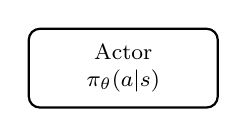
\begin{tikzpicture}[
        box/.style={draw, rounded corners, minimum width=2.4cm,
            minimum height=1.0cm, align=center, thick},
        every node/.style={font=\footnotesize}]
        \node[box] (actor) {Actor\\$\pi_\theta(a|s)$};
        % \node[box, below=1.6cm of actor] (critic)
        %     {Critic\\$V_\phi(s)$};
        % \node[box, right=3.2cm of $(actor)!0.5!(critic)$] (env)
        %     {Περιβάλλον};
        % \draw[-{Stealth[length=2.5mm]}, thick] (actor.east) -- ++(1.0,0) |- (env.west)
        %     node[pos=0.25, above, font=\scriptsize] {$a_t$};
        % \draw[-{Stealth[length=2.5mm]}, thick] (env.west) -- ++(-1.0,0) |- (critic.east)
        %     node[pos=0.75, below, font=\scriptsize] {$s_t, r_t$};
        % \draw[-{Stealth[length=2.5mm]}, thick] (critic.north) -- (actor.south)
        %     node[midway, right, font=\scriptsize] {$A_t$};
    \end{tikzpicture}
    \caption{Αρχιτεκτονική Actor/Critic. Ο Critic εκτιμά την αξία της
    κατάστασης και τροφοδοτεί τον Actor με το σήμα πλεονεκτήματος $A_t$, το
    οποίο κατευθύνει την ενημέρωση της πολιτικής.}
    \label{fig:actor-critic}
\end{figure}

\begin{table}[ht]
    \centering
    \caption{Ταξινόμηση βασικών οικογενειών αλγορίθμων Ενισχυτικής Μάθησης.}
    \label{tab:rl-taxonomy}
    \begin{tabular}{@{}lll@{}}
        \toprule
        \textbf{Οικογένεια} & \textbf{Τι μαθαίνει} & \textbf{Παραδείγματα} \\
        \midrule
        Βασισμένη στην αξία & $Q(s,a)$ & Q-learning, DQN \\
        Βασισμένη στην πολιτική & $\pi_\theta(a\mid s)$ & REINFORCE \\
        Actor/Critic & $\pi_\theta$ \& $V_\phi$ & A2C, A3C, PPO, SAC \\
        \bottomrule
    \end{tabular}
\end{table}


% ---------------------------------------------------------------------
\subsection{Αλγόριθμος Proximal Policy Optimization (PPO)}
\label{subsec:ppo}
% ---------------------------------------------------------------------

Βασικό πρόβλημα των μεθόδων κλίσης πολιτικής είναι ότι μεγάλα βήματα
ενημέρωσης μπορούν να καταστρέψουν μια ήδη καλή πολιτική, οδηγώντας σε
κατάρρευση της απόδοσης. Ο αλγόριθμος \emph{Trust Region Policy Optimization}
(TRPO)~\cite{schulman2015trpo} αντιμετώπισε το ζήτημα περιορίζοντας την
\emph{απόκλιση KL} (Kullback-Leibler divergence,
$D_{\mathrm{KL}}(\pi_{\mathrm{old}} \| \pi_\theta) = \mathbb{E}_{a \sim
\pi_{\mathrm{old}}}\!\left[\log \frac{\pi_{\mathrm{old}}(a \mid s)}{\pi_\theta(a
\mid s)}\right]$), η οποία μετρά πόσο διαφέρει η νέα κατανομή πολιτικής από
την παλαιά, μεταξύ διαδοχικών ενημερώσεων, με κόστος όμως σημαντική
υπολογιστική πολυπλοκότητα.

Ο αλγόριθμος \emph{Proximal Policy Optimization}
(PPO)~\cite{schulman2017ppo} επιτυγχάνει παρόμοια ευστάθεια με δραστικά
απλούστερο τρόπο, χρησιμοποιώντας έναν μηχανισμό \emph{αποκοπής} (clipping). Είναι σήμερα ένας από τους δημοφιλέστερους αλγορίθμους DRL και
αποτελεί τον πυρήνα του πράκτορα της παρούσας εργασίας, λόγω της ευρωστίας του
σε θορυβώδη, μη στάσιμα περιβάλλοντα.

Η συνολική αντικειμενική συνάρτηση του PPO είναι μια \emph{σύνθετη απώλεια}
που συνενώνει τρεις όρους.

\paragraph{1.\ Αποκομμένη υποκατάστατη απώλεια (Actor).}
Έστω ο λόγος πιθανοτήτων μεταξύ νέας και παλαιάς πολιτικής:
\begin{equation}
    r_t(\theta) = \frac{\pi_{\theta}(a_t \mid s_t)}
    {\pi_{\theta_{\mathrm{old}}}(a_t \mid s_t)}.
    \label{eq:ppo-ratio}
\end{equation}
Η απώλεια του Actor ορίζεται ως:
\begin{equation}
    \mathcal{L}^{\mathrm{CLIP}}(\theta) = \mathbb{E}_t\!\Big[
    \min\big( r_t(\theta)\hat{A}_t,\;
    \mathrm{clip}(r_t(\theta), 1-\epsilon, 1+\epsilon)\,\hat{A}_t \big)
    \Big],
    \label{eq:ppo-clip}
\end{equation}
όπου $\epsilon$ (τυπικά $0.1$--$0.2$) είναι η υπερπαράμετρος αποκοπής. Ο όρος
$\min$ μαζί με την αποκοπή αποτρέπει την πολιτική από υπερβολικά μεγάλες
μεταβολές σε ένα μόνο βήμα ενημέρωσης, υλοποιώντας μια «μαλακή» περιοχή
εμπιστοσύνης χωρίς ρητό περιορισμό.

\paragraph{2.\ Απώλεια αξίας (Critic).}
Η εκπαίδευση του Critic ελαχιστοποιεί το τετραγωνικό σφάλμα μεταξύ της εκτίμησης
αξίας και των εμπειρικών αποδόσεων $R_t$:
\begin{equation}
    \mathcal{L}^{\mathrm{VF}}(\phi) = \mathbb{E}_t\!\Big[
    \big( V_{\phi}(s_t) - R_t \big)^2 \Big].
    \label{eq:ppo-vf}
\end{equation}

\paragraph{3.\ Όρος εντροπίας.}
Για τη διασφάλιση επαρκούς εξερεύνησης προστίθεται ένας όρος που ενθαρρύνει
στοχαστικές πολιτικές, μέσω της εντροπίας Shannon
$H$ της κατανομής δράσεων:
\begin{equation}
    \mathcal{L}^{\mathrm{ENT}}(\theta) = \mathbb{E}_t\!\big[
    H\!\left(\pi_{\theta}(\cdot \mid s_t)\right) \big].
    \label{eq:ppo-ent}
\end{equation}

\paragraph{Συνολική αντικειμενική συνάρτηση.}
Η τελική συνάρτηση που μεγιστοποιείται είναι ο γραμμικός συνδυασμός των τριών
όρων:
\begin{equation}
    \mathcal{L}^{\mathrm{total}} = \mathbb{E}_t\!\Big[
    \mathcal{L}^{\mathrm{CLIP}}(\theta)
    - c_1 \mathcal{L}^{\mathrm{VF}}(\phi)
    + c_2 \mathcal{L}^{\mathrm{ENT}}(\theta) \Big],
    \label{eq:ppo-total}
\end{equation}
όπου $c_1, c_2$ είναι συντελεστές στάθμισης. Στην παρούσα εργασία, ο PPO
συνδυάζεται με αναδρομικό δίκτυο LSTM (PPO-LSTM):
η κρυφή κατάσταση τροφοδοτεί τόσο τον Actor όσο και τον Critic, επιτρέποντας τη
λήψη αποφάσεων με βάση το ιστορικό, όπως απαιτεί το μερικώς παρατηρήσιμο
χρηματοοικονομικό περιβάλλον.


% =====================================================================
\section{Μεγάλα Γλωσσικά Μοντέλα και Ανάλυση Συναισθήματος}
\label{sec:llm}
% =====================================================================

Η αποκλειστική χρήση αριθμητικών δεδομένων αγοράς αγνοεί έναν τεράστιο όγκο
πληροφορίας που περιέχεται σε κείμενα: ειδήσεις, οικονομικές αναφορές,
αναρτήσεις σε μέσα κοινωνικής δικτύωσης. Η ενότητα αυτή παρουσιάζει τα Μεγάλα Γλωσσικά Μοντέλα (LLM) και τις
τεχνικές ανάλυσης συναισθήματος.


% ---------------------------------------------------------------------
\subsection{Επεξεργασία Φυσικής Γλώσσας και η Αρχιτεκτονική Transformer}
\label{subsec:nlp-transformer}
% ---------------------------------------------------------------------

Η Επεξεργασία Φυσικής Γλώσσας (Natural Language
Processing, NLP) αποσκοπεί στην υπολογιστική κατανόηση και παραγωγή
ανθρώπινης γλώσσας. Οι πρώιμες προσεγγίσεις βασίστηκαν σε διανυσματικές
αναπαραστάσεις λέξεων (word embeddings), που
απεικονίζουν λέξεις σε έναν συνεχή χώρο όπου η σημασιολογική εγγύτητα
αντιστοιχεί σε γεωμετρική εγγύτητα. Ωστόσο, οι αναπαραστάσεις αυτές ήταν
στατικές, αδυνατώντας να αποτυπώσουν την εξάρτηση της σημασίας από τα
συμφραζόμενα.

Η καθοριστική τομή ήρθε με την αρχιτεκτονική \emph{Transformer} και τον
\emph{Μηχανισμό Αυτο-Προσοχής} (Self-Attention)~\cite{vaswani2017attention}.
Σε αντίθεση με τα αναδρομικά δίκτυα που επεξεργάζονται την ακολουθία διαδοχικά,
η προσοχή επιτρέπει σε κάθε διακριτικό (token) να
«εστιάζει» ταυτόχρονα σε όλα τα υπόλοιπα, υπολογίζοντας σταθμισμένους
συσχετισμούς. Δεδομένων των πινάκων Ερωτημάτων $\mathbf{Q}$, Κλειδιών
$\mathbf{K}$ και Τιμών $\mathbf{V}$, η προσοχή ορίζεται ως:
\begin{equation}
    \mathrm{Attention}(\mathbf{Q}, \mathbf{K}, \mathbf{V}) =
    \mathrm{softmax}\!\left(
    \frac{\mathbf{Q}\mathbf{K}^{\top}}{\sqrt{d_k}}
    \right)\mathbf{V},
    \label{eq:attention}
\end{equation}
όπου $d_k$ είναι η διάσταση των κλειδιών και ο παράγοντας $\sqrt{d_k}$
σταθεροποιεί αριθμητικά τις κλίσεις. Ο μηχανισμός επεκτείνεται σε
\emph{πολλαπλές κεφαλές} (multi-head attention),
που επιτρέπουν την ταυτόχρονη μάθηση διαφορετικών τύπων σχέσεων. Η
παραλληλοποιήσιμη φύση των Transformers κατέστησε εφικτή την κλιμάκωση σε
μοντέλα δισεκατομμυρίων παραμέτρων.

\paragraph{Θεωρητική δικαιολόγηση και επιλογή για χρηματοοικονομικό κείμενο.}
Η υπεροχή των Transformers έναντι των κλασικών αναδρομικών δικτύων στη
μοντελοποίηση κειμένου ερείδεται σε δύο θεωρητικές ιδιότητες: αφενός, ο
μηχανισμός αυτο-προσοχής παρέχει \emph{άμεση} σύνδεση μεταξύ κάθε ζεύγους
διακριτικών, ανεξαρτήτως απόστασης στην ακολουθία, αποφεύγοντας το πρόβλημα
της εξασθένισης κλίσης που πλήττει τα RNN. Αφετέρου, η παραλληλοποίηση του
υπολογισμού επιτρέπει αποδοτική εκπαίδευση σε τεράστια σώματα κειμένων, από τα
οποία το μοντέλο αναδύει ισχυρές αναπαραστάσεις συμφραζομένων. Αυτές οι
ιδιότητες είναι ιδιαιτέρως σχετικές για το χρηματοοικονομικό πεδίο: η
σημαντικότητα μιας ειδησεογραφικής φράσης συχνά εξαρτάται από το ευρύτερο
πλαίσιό της (π.χ.\ η λέξη «αθέτηση» φέρει διαφορετικό συναισθηματικό φορτίο
σε κειμενικό περιβάλλον που αφορά κρατικό χρέος έναντι τεχνολογικής ορολογίας),
κάτι που τα στατικά λεξικά ή οι αναπαραστάσεις χωρίς συμφραζόμενα δεν μπορούν
να αποτυπώσουν.

\paragraph{Περιορισμοί και γνωστά αδύναμα σημεία.}
Παρά την εμπειρική επιτυχία τους, οι Transformers εμφανίζουν ορισμένους
γνωστούς περιορισμούς που είναι συναφείς για την εφαρμογή τους σε
χρηματοοικονομικά κείμενα. Πρώτον, η πολυπλοκότητα της αυτο-προσοχής
κλιμακώνεται τετραγωνικά ως προς το μήκος της ακολουθίας, γεγονός που
περιορίζει την άμεση επεξεργασία πολύ μακρών εγγράφων (π.χ.\ εκτενείς εκθέσεις
αποτελεσμάτων). Δεύτερον, η προεκπαίδευση σε γενικά κείμενα δεν εγγυάται
επαρκή κατανόηση της εξειδικευμένης ορολογίας των κρυπτονομισμάτων, η οποία
εξελίσσεται ταχύτατα και περιλαμβάνει ιδιαίτερες εκφράσεις της κοινότητας
(π.χ.\ «FOMO», «rug pull», «whale alert»). Αυτός ακριβώς ο περιορισμός
δικαιολογεί τη μικρο-προσαρμογή (fine-tuning) του LLM σε στοχευμένα δεδομένα
χρηματοοικονομικής ειδησεογραφίας, η οποία αναλύεται στην
Ενότητα~\ref{subsec:lora}.


% ---------------------------------------------------------------------
\subsection{Μεγάλα Γλωσσικά Μοντέλα (LLMs)}
\label{subsec:llm}
% ---------------------------------------------------------------------

Τα \emph{Μεγάλα Γλωσσικά Μοντέλα} (Large Language
Models, LLMs) είναι μοντέλα βασισμένα σε Transformers με εκατομμύρια έως
δισεκατομμύρια παραμέτρους, εκπαιδευμένα σε τεράστια σώματα κειμένων. Η
εκπαίδευσή τους ακολουθεί τυπικά δύο φάσεις:
\begin{enumerate}
    \item \textbf{Προεκπαίδευση} (pre-training):
    αυτο-επιβλεπόμενη μάθηση σε γενικά κείμενα, με στόχο την πρόβλεψη του
    επόμενου διακριτικού (autoregressive language
    modeling, π.χ.\ μοντέλα τύπου GPT~\cite{brown2020gpt3})
    ή την ανακατασκευή αποκρυμμένων διακριτικών
    (masked language modeling, π.χ.\
    BERT~\cite{devlin2019bert}).
    \item \textbf{Μικρο-προσαρμογή} (fine-tuning):
    εξειδίκευση του προεκπαιδευμένου μοντέλου σε μια συγκεκριμένη εργασία ή
    πεδίο με μικρότερο, στοχευμένο σύνολο δεδομένων.
\end{enumerate}

Τα LLMs επιδεικνύουν αξιοσημείωτες ικανότητες \emph{μηδενικής}
(zero-shot) και \emph{ολίγων δειγμάτων}
(few-shot) μάθησης, καθώς και αναδυόμενη
συλλογιστική ικανότητα. Στο χρηματοοικονομικό πεδίο, μπορούν να αναλύσουν τη
σημασιολογία ειδήσεων και αναρτήσεων, εξάγοντας δείκτες επενδυτικής
ψυχολογίας.


% ---------------------------------------------------------------------
\subsection{Ανάλυση Συναισθήματος}
\label{subsec:sentiment}
% ---------------------------------------------------------------------

Η \emph{Ανάλυση Συναισθήματος} (Sentiment Analysis)
είναι η εργασία NLP που στοχεύει στον προσδιορισμό της συναισθηματικής
χροιάς ενός κειμένου, τυπικά σε μια κλίμακα θετικό/ουδέτερο/αρνητικό ή σε μια
συνεχή βαθμολογία. Η ιστορική της εξέλιξη διακρίνεται σε τρεις γενιές:
\begin{enumerate}
    \item \textbf{Μέθοδοι λεξικού} (lexicon-based):
    βασίζονται σε προκαθορισμένα λεξικά λέξεων με συναισθηματικά φορτία. Στα
    χρηματοοικονομικά, σταθμός υπήρξε το λεξικό
    Loughran/McDonald~\cite{loughran2011}, που
    προσάρμοσε την ανάλυση στην ιδιαίτερη ορολογία των οικονομικών αναφορών.
    Αδυναμία τους η αδυναμία σύλληψης συμφραζομένων, άρνησης και σαρκασμού.
    \item \textbf{Μέθοδοι μηχανικής μάθησης / Transformers}: μοντέλα όπως το
    FinBERT~\cite{araci2019finbert}, ένα
    BERT προσαρμοσμένο σε χρηματοοικονομικά κείμενα,
    παρέχουν αναπαραστάσεις ευαίσθητες στα συμφραζόμενα, βελτιώνοντας
    δραστικά την ακρίβεια.
    \item \textbf{Μέθοδοι βασισμένες σε LLM}: αναλύονται στην επόμενη
    υποενότητα.
\end{enumerate}


% ---------------------------------------------------------------------
\subsection{Ανάλυση Συναισθήματος με LLM}
\label{subsec:llm-sentiment}
% ---------------------------------------------------------------------

Τα σύγχρονα LLMs μετατόπισαν το πεδίο της ανάλυσης συναισθήματος. Μοντέλα όπως
οι παραλλαγές των LLaMA και GPT,
και εξειδικευμένα χρηματοοικονομικά μοντέλα όπως το
FinGPT~\cite{yang2023fingpt}, επιτυγχάνουν ανώτερη
ακρίβεια χάρη στη βαθιά κατανόηση συμφραζομένων και την ικανότητα
συλλογιστικής. Αντί απλής ταξινόμησης, ένα LLM μπορεί να παραγάγει μια
βαθμολογημένη εκτίμηση συναισθήματος συνοδευόμενη ακόμη και από αιτιολόγηση.

Στην παρούσα εργασία, ένα LLM προσαρμόζεται στη χρηματοοικονομική/επενδυτική
γλώσσα ώστε να εξάγει έναν \emph{αριθμητικό δείκτη συναισθήματος} που να είναι
σταθερός, αναπαραγώγιμος και συγχρονισμένος με τα χρονικά βήματα της αγοράς.
Ο δείκτης αυτός αξιοποιείται διττά από τον πράκτορα DRL: αφενός ως πρόσθετο
χαρακτηριστικό της κατάστασης, αφετέρου ως μηχανισμός προσαρμογής της έντασης
των ενεργειών. Η ενσωμάτωση LLM-σημάτων συναισθήματος ως εξωγενών μεταβλητών σε
συστήματα DRL αποτελεί ανοιχτό ερευνητικό ζήτημα, με κεντρικό πρόβλημα τον
βέλτιστο τρόπο σύντηξης (data fusion) κειμενικής και
αριθμητικής πληροφορίας.


% ---------------------------------------------------------------------
\subsection{Αποδοτική Μικρο-προσαρμογή: Low-Rank Adaptation (LoRA)}
\label{subsec:lora}
% ---------------------------------------------------------------------

Η πλήρης μικρο-προσαρμογή (full fine-tuning) ενός
LLM, που ενημερώνει το σύνολο των δισεκατομμυρίων παραμέτρων, είναι
υπολογιστικά απαγορευτική για τους περισσότερους ερευνητές, λόγω των τεράστιων
απαιτήσεων μνήμης GPU. Οι τεχνικές \emph{Αποδοτικής ως προς τις Παραμέτρους
Μικρο-προσαρμογής} (Parameter-Efficient Fine-Tuning,
PEFT) αντιμετωπίζουν το πρόβλημα ενημερώνοντας μόνο ένα μικρό υποσύνολο
παραμέτρων.

Η σημαντικότερη μέθοδος PEFT είναι η \emph{Προσαρμογή Χαμηλής Βαθμίδας}
(Low-Rank Adaptation, LoRA)~\cite{hu2021lora}. Η
βασική ιδέα στηρίζεται στην παρατήρηση ότι η μεταβολή των βαρών κατά τη
μικρο-προσαρμογή έχει χαμηλή «εγγενή βαθμίδα»
(intrinsic rank). Έτσι, αντί να ενημερώνεται ο
πλήρης πίνακας βαρών $\mathbf{W}_0 \in \mathbb{R}^{d \times k}$, αυτός
παγώνει και η μεταβολή $\Delta\mathbf{W}$ αναπαρίσταται ως γινόμενο δύο πολύ
μικρότερων πινάκων:
\begin{equation}
    \mathbf{W} = \mathbf{W}_0 + \Delta\mathbf{W}
    = \mathbf{W}_0 + \mathbf{B}\mathbf{A},
    \label{eq:lora}
\end{equation}
όπου $\mathbf{B} \in \mathbb{R}^{d \times r}$,
$\mathbf{A} \in \mathbb{R}^{r \times k}$ και η βαθμίδα $r \ll \min(d, k)$.
Κατά την εκπαίδευση, εν προκειμένω σε δεδομένα χρηματοοικονομικού
συναισθήματος, ενημερώνονται μόνο οι πίνακες $\mathbf{A}$ και $\mathbf{B}$,
μειώνοντας τον αριθμό των εκπαιδεύσιμων παραμέτρων κατά τάξεις μεγέθους και
περιορίζοντας δραστικά τις απαιτήσεις μνήμης, χωρίς ουσιαστική απώλεια
ακρίβειας. Επιπλέον, καθώς το $\mathbf{W}_0$ παραμένει αναλλοίωτο, για κάθε εξειδίκευση
χρειάζεται να αποθηκευτούν μόνο οι δύο μικροί πίνακες $\mathbf{A}$ και
$\mathbf{B}$, και όχι ένα πλήρες αντίγραφο του βασικού μοντέλου. Αυτό σημαίνει
ότι διαφορετικά σύνολα LoRA παραμέτρων, εκπαιδευμένα για διαφορετικές εργασίες
ή πεδία (π.χ.\ ανάλυση συναισθήματος κρυπτονομισμάτων έναντι παραδοσιακών
μετοχών), μπορούν να εναλλάσσονται δυναμικά κατά τη διάρκεια της εξαγωγής
συμπερασμάτων, απλώς αντικαθιστώντας τους πίνακες $\mathbf{A}$ και $\mathbf{B}$,
χωρίς καμία μεταβολή στα παγωμένα βάρη $\mathbf{W}_0$. Αυτή η ιδιότητα
καθιστά τη LoRA ιδιαιτέρως ελκυστική για σενάρια πολλαπλών εξειδικεύσεων σε
περιορισμένη υπολογιστική υποδομή, όπως είναι η παρούσα εφαρμογή.


% =====================================================================
\section{Χρηματοοικονομικές Συναλλαγές}
\label{sec:finance}
% =====================================================================

Η τελευταία ενότητα του θεωρητικού υποβάθρου εισάγει τις έννοιες των
χρηματοοικονομικών αγορών που είναι απαραίτητες για τη διατύπωση του
προβλήματος ως διαδικασίας λήψης αποφάσεων, καθώς και τα μέτρα αξιολόγησης της
απόδοσης ενός πράκτορα συναλλαγών.


% ---------------------------------------------------------------------
\subsection{Βασικές Έννοιες στις Χρηματοοικονομικές Αγορές}
\label{subsec:market-basics}
% ---------------------------------------------------------------------

Μια \emph{χρηματοοικονομική αγορά} είναι ένας μηχανισμός όπου αγοραστές και
πωλητές ανταλλάσσουν \emph{περιουσιακά στοιχεία}
(assets), μετοχές, ομόλογα, συνάλλαγμα,
κρυπτονομίσματα. Η \emph{τιμή} ενός στοιχείου διαμορφώνεται από τη
δυναμική προσφοράς και ζήτησης. Θεμελιώδεις έννοιες είναι:
\begin{itemize}
    \item \textbf{Τιμές προσφοράς/ζήτησης}
    (bid/ask): η υψηλότερη τιμή που είναι
    διατεθειμένος να πληρώσει ένας αγοραστής (bid)
    και η χαμηλότερη που δέχεται ένας πωλητής
    (ask). Η διαφορά τους είναι το
    \emph{περιθώριο} (spread).
    \item \textbf{Ρευστότητα} (liquidity): η
    ευκολία αγοραπωλησίας χωρίς σημαντική επίδραση στην τιμή.
    \item \textbf{Βιβλίο εντολών} (order book): η
    συγκεντρωτική καταγραφή των ενεργών εντολών αγοράς και πώλησης.
    \item \textbf{Μεταβλητότητα} (volatility): η
    έκταση των διακυμάνσεων της τιμής, τυπικά μετρούμενη ως η τυπική απόκλιση
    των αποδόσεων.
\end{itemize}

Η \emph{χρηματοοικονομική απόδοση} (financial return) ενός στοιχείου μεταξύ
δύο διαδοχικών χρονικών στιγμών ορίζεται είτε ως απλή ποσοστιαία μεταβολή είτε
ως λογαριθμική απόδοση:
\begin{equation}
    r_t = \frac{P_t - P_{t-1}}{P_{t-1}},
    \qquad
    r_t^{\log} = \ln\!\left(\frac{P_t}{P_{t-1}}\right).
    \label{eq:returns}
\end{equation}
Οι λογαριθμικές αποδόσεις προτιμώνται λόγω της ιδιότητας της χρονικής
προσθετικότητας. Διευκρινίζεται ότι η έννοια αυτή είναι διαφορετική από την
\emph{απόδοση} της Ενισχυτικής Μάθησης (return στην ορολογία RL, ορισμός
στην Ενότητα~\ref{subsec:mdp}), η οποία εκφράζει τη \emph{σωρευτική
προεξοφλημένη ανταμοιβή} $G_t = \sum_{k=0}^{\infty} \gamma^k r_{t+k+1}$ και
αποτελεί λογιστμική ποσότητα που χρησιμοποιείται για τη βελτιστοποίηση της
πολιτικής, όχι μέτρο της μεταβολής τιμής. Στην παρούσα εργασία, η χρηματοοικονομική
απόδοση $r_t$ αποτελεί τη βάση του σήματος ανταμοιβής που λαμβάνει ο
πράκτορας, ενώ ο στόχος βελτιστοποίησης είναι η RL απόδοση $G_t$.

\paragraph{Υπόθεση Αποτελεσματικής Αγοράς.}
Η \emph{Υπόθεση Αποτελεσματικής Αγοράς} (Efficient
Market Hypothesis, EMH)~\cite{fama1970emh} υποστηρίζει ότι οι τιμές
ενσωματώνουν άμεσα όλη τη διαθέσιμη πληροφορία, καθιστώντας θεωρητικά αδύνατη
τη σταθερή υπεραπόδοση. Η \emph{ημι-ισχυρή} μορφή της υποδεικνύει ότι οι τιμές
προσαρμόζονται ταχύτατα στις νέες δημόσιες πληροφορίες, οι οποίες όμως συχνά
εμφανίζονται πρώτα σε κειμενική μορφή, γεγονός που θεμελιώνει τη χρησιμότητα
της ανάλυσης συναισθήματος. Παρά την επιρροή της EMH, η συμπεριφορική
χρηματοοικονομική τεκμηριώνει συστηματικές αναποτελεσματικότητες οφειλόμενες σε
ψυχολογικούς παράγοντες, ιδίως σε αγορές υψηλής κερδοσκοπίας και λιανικής
συμμετοχής όπως τα κρυπτονομίσματα.


% ---------------------------------------------------------------------
\subsection{Χρηματοοικονομικά Δεδομένα, Κεριά και Θέσεις}
\label{subsec:data-candles}
% ---------------------------------------------------------------------

\paragraph{Δεδομένα OHLCV και κεριά.}
Στην πράξη, τα δεδομένα τιμών συγκεντρώνονται σε διακριτά χρονικά διαστήματα
(π.χ.\ λεπτό, ώρα, ημέρα) και αναπαρίστανται με τη μορφή \emph{OHLCV}:
τιμή ανοίγματος (Open), υψηλότερη
(High), χαμηλότερη (Low),
κλεισίματος (Close) και όγκος συναλλαγών
(Volume). Κάθε τέτοια εγγραφή απεικονίζεται οπτικά
ως ένα \emph{κερί} (candlestick)
(Σχήμα~\ref{fig:candlestick}): το «σώμα» εκτείνεται μεταξύ ανοίγματος και
κλεισίματος, ενώ οι «σκιές» φτάνουν στη μέγιστη και ελάχιστη τιμή. Ένα πράσινο
(ανοδικό) κερί υποδηλώνει κλείσιμο υψηλότερο του ανοίγματος, ένα κόκκινο
(πτωτικό) το αντίθετο.

\begin{figure}[ht]
    \centering
    \begin{tikzpicture}[every node/.style={font=\scriptsize}]
        % bullish candle
        \draw[thick] (0,0.3) -- (0,3.2);          % lower-upper wick
        \draw[very thick, fill=white] (-0.25,1.0) rectangle (0.25,2.6);
        \node at (0,-0.2) {ανοδικό};
        \node[right] at (0.35,2.6) {Κλείσιμο};
        \node[right] at (0.35,1.0) {Άνοιγμα};
        \node[right] at (0.35,3.2) {High};
        \node[right] at (0.35,0.3) {Low};
        % bearish candle
        \begin{scope}[xshift=4.2cm]
            \draw[thick] (0,0.3) -- (0,3.2);
            \draw[very thick, fill=black!25] (-0.25,1.2) rectangle (0.25,2.4);
            \node at (0,-0.2) {πτωτικό};
            \node[right] at (0.35,2.4) {Άνοιγμα};
            \node[right] at (0.35,1.2) {Κλείσιμο};
            \node[right] at (0.35,3.2) {High};
            \node[right] at (0.35,0.3) {Low};
        \end{scope}
    \end{tikzpicture}
    \caption{Δομή ενός ανοδικού (αριστερά) και ενός πτωτικού (δεξιά) κεριού.
    Το σώμα ορίζεται από το άνοιγμα και το κλείσιμο, ενώ οι σκιές δείχνουν το
    εύρος υψηλότερης--χαμηλότερης τιμής εντός του διαστήματος.}
    \label{fig:candlestick}
\end{figure}

\paragraph{Θέσεις.}
Μια \emph{θέση} (position) εκφράζει την έκθεση του
συναλλασσόμενου σε ένα στοιχείο. Διακρίνονται:
\begin{itemize}
    \item \textbf{Θέση αγοράς} (long): ο
    συναλλασσόμενος κατέχει το στοιχείο και επωφελείται από άνοδο της τιμής.
    \item \textbf{Θέση πώλησης} (short): ο
    συναλλασσόμενος έχει δανειστεί και πουλήσει το στοιχείο, επωφελούμενος από
    πτώση της τιμής.
    \item \textbf{Ουδέτερη θέση} (flat): καμία
    έκθεση στην αγορά.
\end{itemize}
Στον προτεινόμενο πράκτορα, ο χώρος δράσεων αντιστοιχεί ακριβώς στη ρύθμιση
αυτής της θέσης (π.χ.\ άνοιγμα, κλείσιμο ή προσαρμογή του μεγέθους μιας
θέσης), ενώ η κατάσταση του περιβάλλοντος περιλαμβάνει την τρέχουσα θέση μαζί
με τα χαρακτηριστικά της αγοράς και το σήμα συναισθήματος.


% ---------------------------------------------------------------------
\subsection{Κέρδος και Ζημία (Profit and Loss)}
\label{subsec:pnl}
% ---------------------------------------------------------------------

Το \emph{Κέρδος και Ζημία} (Profit and Loss, PnL)
είναι το θεμελιώδες μέτρο της απόδοσης μιας συναλλακτικής δραστηριότητας.
Διακρίνεται σε \emph{μη πραγματοποιημένο}
(unrealized), που αφορά ανοιχτές θέσεις
αποτιμημένες στην τρέχουσα τιμή, και \emph{πραγματοποιημένο}
(realized), που αποκρυσταλλώνεται με το κλείσιμο
μιας θέσης. Για μια θέση μεγέθους $q$ που ανοίγει στην τιμή $P_{\mathrm{in}}$
και κλείνει στην $P_{\mathrm{out}}$, το ακαθάριστο PnL είναι:
\begin{equation}
    \mathrm{PnL} = q\,(P_{\mathrm{out}} - P_{\mathrm{in}}),
    \label{eq:pnl-gross}
\end{equation}
με $q > 0$ για θέση αγοράς και $q < 0$ για θέση πώλησης.

Κρισίμως, η πραγματική απόδοση πρέπει να αφαιρεί τα \emph{κόστη συναλλαγών}
(transaction costs)/προμήθειες, περιθώριο
bid/ask και \emph{ολίσθηση}
(slippage), δηλαδή τη διαφορά μεταξύ αναμενόμενης
και πραγματικής τιμής εκτέλεσης. Το καθαρό PnL για μια ακολουθία συναλλαγών
γίνεται:
\begin{equation}
    \mathrm{PnL}_{\mathrm{net}}
    = \sum_{t} q_t\,(P_{\mathrm{out},t} - P_{\mathrm{in},t})
    - \sum_{t} c\,\lvert \Delta q_t \rvert P_t,
    \label{eq:pnl-net}
\end{equation}
όπου $c$ είναι ο αναλογικός συντελεστής κόστους ανά συναλλαγή. Η ενσωμάτωση
αυτών των κοστών είναι απαραίτητη: μια στρατηγική κερδοφόρα σε θεωρητικό
επίπεδο μπορεί να καταστεί ζημιογόνα μόλις ληφθούν υπόψη τα κόστη υψηλής
συχνότητας συναλλαγών. Στον πράκτορα DRL, το καθαρό PnL αποτελεί τη βάση της
συνάρτησης ανταμοιβής, η οποία μπορεί επιπλέον να ενσωματώνει όρους ποινής για
τον κίνδυνο.


% ---------------------------------------------------------------------
\subsection{Ενεργό Κέρδος (Alpha) και Μέτρα Προσαρμοσμένα στον Κίνδυνο}
\label{subsec:alpha}
% ---------------------------------------------------------------------

Η αξιολόγηση μιας στρατηγικής με βάση μόνο το απόλυτο κέρδος είναι παραπλανητική,
καθώς αγνοεί τόσο τον αναλαμβανόμενο κίνδυνο όσο και την απόδοση που θα
προέκυπτε από μια παθητική επένδυση στην αγορά.

\paragraph{Ενεργό κέρδος (alpha).}
Το \emph{ενεργό κέρδος} ή \emph{άλφα} (alpha,
$\alpha$) μετρά την υπερβάλλουσα απόδοση μιας στρατηγικής πέραν εκείνης που
δικαιολογείται από την έκθεσή της στον συστηματικό κίνδυνο της αγοράς. Με βάση
το Υπόδειγμα Αποτίμησης Κεφαλαιουχικών Στοιχείων
(CAPM), η αναμενόμενη απόδοση ενός χαρτοφυλακίου
$p$ διατυπώνεται ως:
\begin{equation}
    \mathbb{E}[r_p] = r_f + \beta_p\big(\mathbb{E}[r_m] - r_f\big) + \alpha,
    \label{eq:alpha}
\end{equation}
όπου $r_f$ η απόδοση χωρίς κίνδυνο, $r_m$ η απόδοση της αγοράς και $\beta_p$ ο
συντελεστής συστηματικού κινδύνου~\cite{jensen1968alpha}. Θετικό $\alpha$
υποδηλώνει ότι η στρατηγική παράγει αξία πέρα από την απλή έκθεση στην αγορά, 
ακριβώς ο στόχος ενός ευφυούς πράκτορα συναλλαγών.

\paragraph{Μέτρα προσαρμοσμένα στον κίνδυνο.}
Για την ολοκληρωμένη αξιολόγηση χρησιμοποιούνται μέτρα που σταθμίζουν την
απόδοση με τον κίνδυνο (Πίνακας~\ref{tab:metrics}). Ο \emph{Λόγος Sharpe}
(Sharpe Ratio)~\cite{sharpe1966} είναι ο
πλέον διαδεδομένος:
\begin{equation}
    \mathrm{Sharpe} = \frac{\mathbb{E}[r_p] - r_f}{\sigma_p},
    \label{eq:sharpe}
\end{equation}
όπου $\sigma_p$ η τυπική απόκλιση των αποδόσεων. Ο \emph{Λόγος Sortino}
αντικαθιστά την $\sigma_p$ με την απόκλιση μόνο των αρνητικών αποδόσεων
(downside deviation), τιμωρώντας μόνο τον
ανεπιθύμητο κίνδυνο. Η \emph{Μέγιστη Πτώση Κεφαλαίου}
(Maximum Drawdown) μετρά τη μεγαλύτερη σωρευτική
απώλεια από μια κορυφή έως μια κοιλάδα και αποτυπώνει τον κίνδυνο
καταστροφικών ζημιών.

\begin{table}[ht]
    \centering
    \caption{Βασικά μέτρα αξιολόγησης απόδοσης στρατηγικών συναλλαγών.}
    \label{tab:metrics}
    \begin{tabular}{@{}lll@{}}
        \toprule
        \textbf{Μέτρο} & \textbf{Τι μετρά} & \textbf{Επιθυμητή τιμή} \\
        \midrule
        Sharpe Ratio & απόδοση ανά μονάδα συνολικού κινδύνου & υψηλή \\
        Sortino Ratio & απόδοση ανά μονάδα αρνητικού κινδύνου & υψηλή \\
        Max Drawdown & μέγιστη σωρευτική απώλεια & χαμηλή (απ.\ τιμή) \\
        $\alpha$ (alpha) & υπεραπόδοση έναντι αγοράς & θετική \\
        Calmar Ratio & απόδοση ανά μονάδα μέγ.\ πτώσης & υψηλή \\
        \bottomrule
    \end{tabular}
\end{table}

Στην παρούσα εργασία, τα μέτρα αυτά χρησιμεύουν τόσο για την αντικειμενική
σύγκριση του προτεινόμενου πράκτορα με σημεία αναφοράς
(baselines), όσο και, ενδεχομένως, ως συστατικά
της συνάρτησης ανταμοιβής, ώστε ο πράκτορας να ενθαρρύνεται όχι απλώς να
κερδίζει, αλλά να κερδίζει με ελεγχόμενο κίνδυνο.


% ---------------------------------------------------------------------
\subsection{Τεχνητή Νοημοσύνη στις Συναλλαγές}
\label{subsec:ai-trading}
% ---------------------------------------------------------------------

Η εφαρμογή DRL στις αγορές κρυπτονομισμάτων παρουσιάζει ορισμένες ιδιαιτέρως
απαιτητικές προκλήσεις που δεν αντιμετωπίζονται επαρκώς στη βιβλιογραφία
παραδοσιακών αγορών~\cite{moody2001rltrading,deng2016drltrading}. Κεντρικό
ζήτημα είναι η \emph{μη στασιμότητα}: οι αγορές κρυπτονομισμάτων λειτουργούν
24/7 και υπόκεινται σε απότομες μεταβολές καθεστώτος (regime shifts), στις
οποίες στατιστικές ιδιότητες των δεδομένων, όπως η μεταβλητότητα και οι
συσχετίσεις μεταξύ στοιχείων, μεταβάλλονται ριζικά. Ένας πράκτορας εκπαιδευμένος
σε μια περίοδο bull market ενδέχεται να αποτύχει κατάφωρα υπό συνθήκες bear market
ή και αντιστρόφως, κάτι που επιβάλλει τη χρήση μεθόδων αξιολόγησης που
ελέγχουν ρητά τη γενίκευση διαχρονικά.

Δεύτερη ιδιαιτερότητα είναι ο κίνδυνος \emph{υπερπροσαρμογής στο παρελθόν}
(backtest overfitting)~\cite{lopezdeprado2018}: ο υπερπαραμετρικός χώρος των DRL
πρακτόρων είναι τόσο μεγάλος ώστε να υπάρχει σημαντικός κίνδυνος επιλογής
υπερπαραμέτρων που αξιοποιούν ιδιοσυγκρασίες του ιστορικού δείγματος εκπαίδευσης
χωρίς πραγματική γενικευσιμότητα. Συνδεόμενο με αυτό είναι το πρόβλημα της
\emph{διαρροής μελλοντικής πληροφορίας} (look-ahead bias), στο οποίο
χαρακτηριστικά ή σήματα που κατασκευάζονται στο παρόν χρησιμοποιούν άθελα
μελλοντικά δεδομένα κατά τη φάση του backtest. Ιδιαίτερη επιφυλακή απαιτείται
για τα σήματα συναισθήματος που προέρχονται από LLM: εάν τα δεδομένα κειμένου δεν
ευθυγραμμίζονται με ακρίβεια στο χρόνο με τις τιμές της αγοράς, εισάγεται
συστηματικό look-ahead bias.

Στην παρούσα εργασία, και οι δύο κίνδυνοι αντιμετωπίζονται με τη χρήση
Combinatorial Purged Cross-Validation (CPCV)~\cite{lopezdeprado2018}, μιας
μεθόδου που ειδικά σχεδιάστηκε για χρονοσειρές και επιβάλλει εμπάργκο μεταξύ
ζωνών εκπαίδευσης και επαλήθευσης, εξαλείφοντας τις διαρροές πληροφορίας. Η
βελτιστοποίηση υπερπαραμέτρων διεξάγεται ολοκληρωτικά εντός της CPCV διαδικασίας,
ενώ η τελική αξιολόγηση πραγματοποιείται σε αυστηρά διαχωρισμένο χρονικό τμήμα
(2024-2025) που δεν χρησιμοποιήθηκε σε κανένα στάδιο της εκπαίδευσης ή επιλογής
μοντέλου. Η ακριβής μεθοδολογία αξιολόγησης παρουσιάζεται στο επόμενο κεφάλαιο.

%% --- ΤΕΛΟΣ ΚΕΦΑΛΑΙΟΥ 3 ---